\documentclass[12pt,a4paper]{article}
\usepackage[utf8]{inputenc}
\usepackage[english]{babel}
\usepackage[english]{isodate}
\usepackage[parfill]{parskip}
\usepackage{graphicx}
\usepackage{natbib}
\usepackage{hyperref}
\usepackage{amsmath}
\usepackage{amssymb}
\usepackage{multirow}
\usepackage{float}
\usepackage{rotating}
\usepackage{array}


%opening
\title{\textbf{PhenStat}: \\ statistical analysis of phenotypic data using Linear Mixed Models and Fisher Exact Test\\ \textbf{User's Guide}}
\author{Natalja Kurbatova, Natasha Karp, Jeremy Mason}
\date{Last revised: \today}

\begin{document}
\maketitle
\newpage
\tableofcontents
\newpage
\section{Introduction}
High-throughput phenotyping generates large volumes of varied data including both categorical and continuous data. Operational and cost constraints can lead to a work-flow that precludes traditional analysis methods. Furthermore, for a high throughput environment, a robust automated statistical pipeline that alleviates manual intervention is required. 

PhenStat is a package that provides statistical methods for the identification of abnormal phenotypes with an emphasize on high-throughput dataflows. The package contains dataset checks and cleaning in preparation for the analysis. For continuous data, an iterative fitting process is used to fit a regression model that is the most appropriate for the data (Mixed Model framework), whilst for categorical data, a Fisher Exact Test is implemented (Fisher Exact Test framework). 

Both analysis frameworks output a statistical significance measure, an effect size measure, model diagnostics (when appropriate), and graphical visualisation of the genotype effect. 

The Mixed Model (MM) framework is an iterative process to select the best model for the data which considers both the best modelling approach (mixed model or general linear regression) and which factors to include in the model. There is also user control functionality on whether to include body weight in the modelling process. 

Depending on the user needs, the statistical analysis output can either be interactive where the user can view the graphical output and analysis summary or for a database implementation the output consists of a vector of output and saved graphical files. 

This package has been tested and demonstrated with an application of 420 lines of historic mouse phenotyping data from the  \href{http://www.sanger.ac.uk/mouseportal/}{Sanger MGP} and \href{http://www.europhenome.org/}{Europhenome} resources. 
\\

\begin{figure}[!htpb]%figure01
\centerline{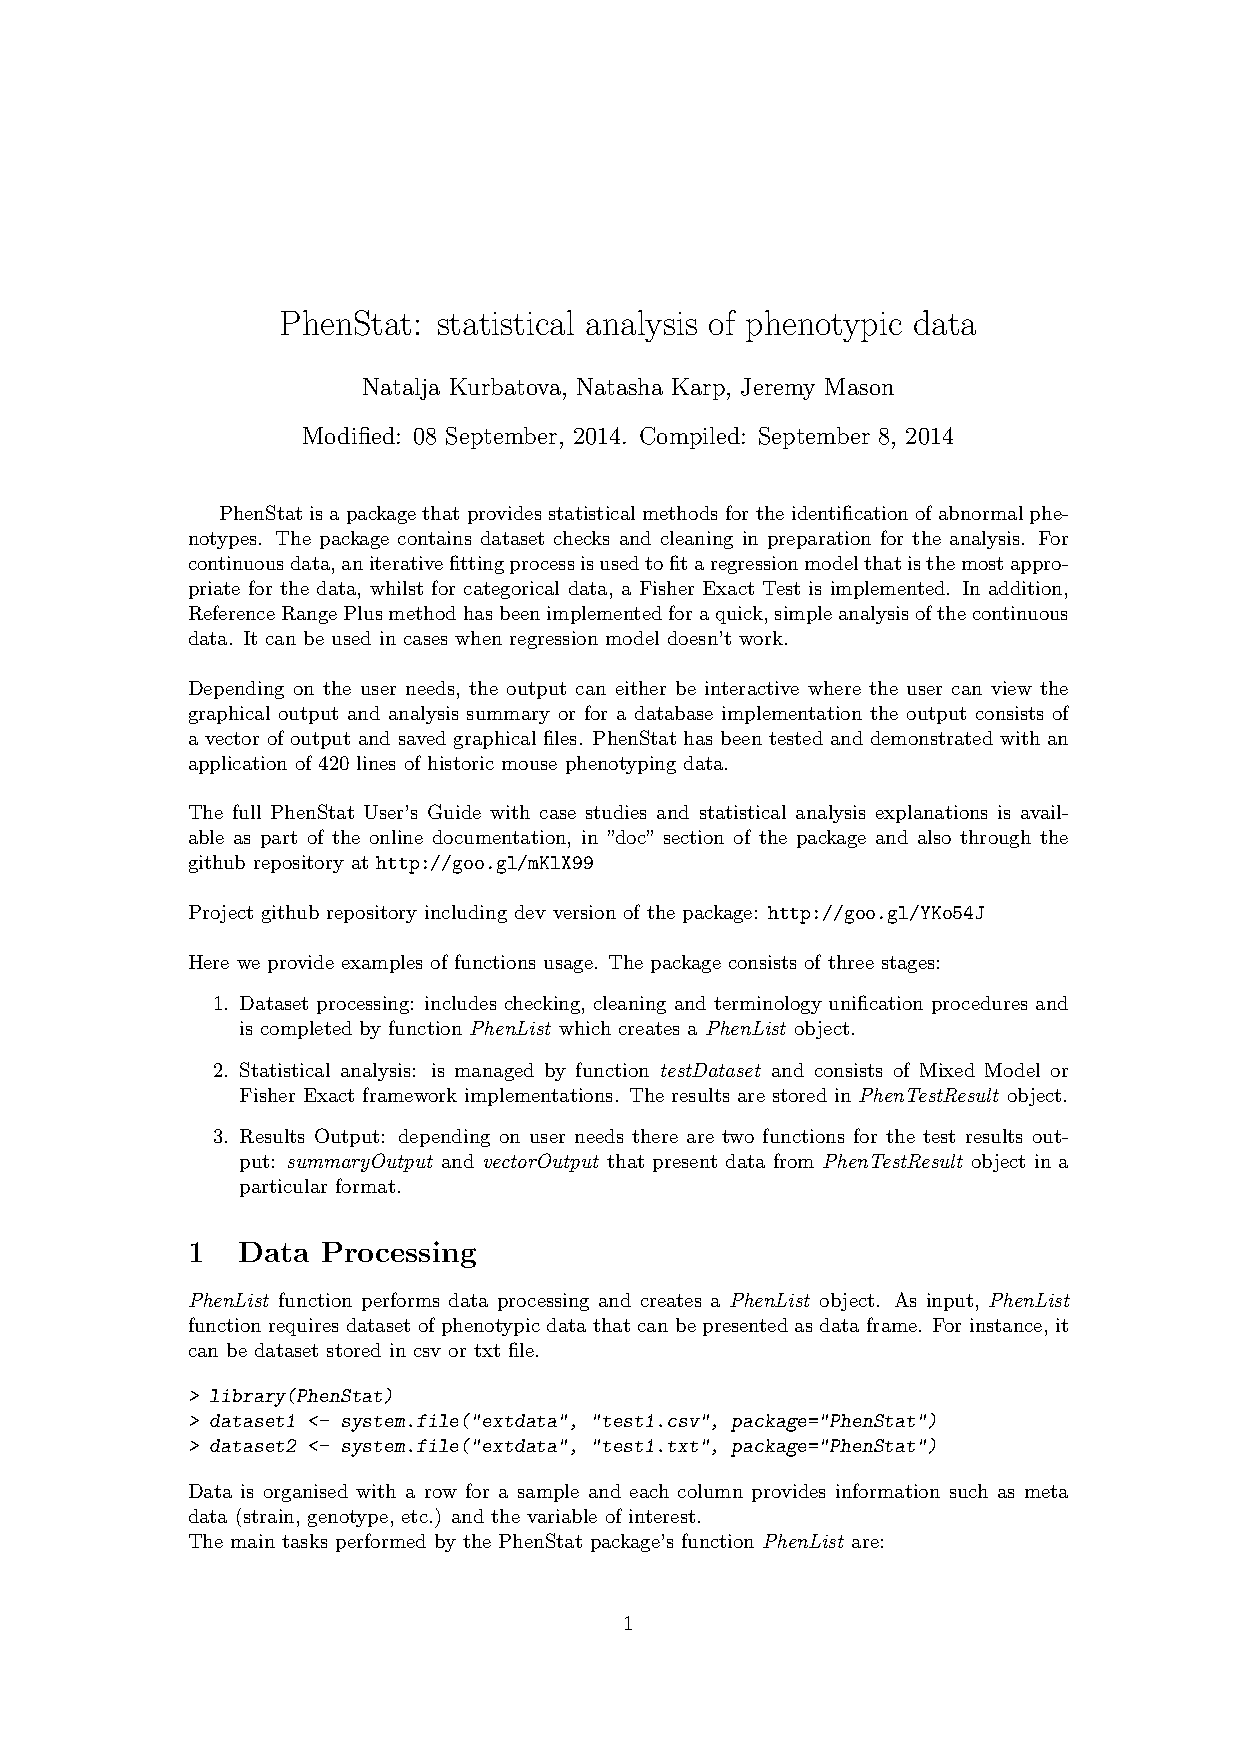
\includegraphics[scale=0.5]{PhenStat.png}}
\caption{The PhenStat package's three stage structure: dataset processing, analysis, and result output. Dotted boxes show the place-holders for new functions that could implement other methods for data analysis and/or output of results.}\label{fig:01}
\end{figure}

The package consists of three stages as shown in Figure \ref{fig:01}:
\begin{enumerate}
\item Dataset processing: includes checking, cleaning and terminology unification procedures and is completed by function \textit{PhenList} which creates a \textit{PhenList} object. 
\item Statistical analysis: is managed by function \textit{testDataset} and consists of Mixed Model or Fisher Exact framework implementations. The results are stored in \textit{PhenTestResult} object. 
Potentially this layer can be extended adding new statistical methods (dotted box in Figure \ref{fig:01}). 
\item Results Output: depending on user needs there are two functions for the test results output: \textit{summaryOutput} 
and \textit{vectorOutput} that present data from \textit{PhenTestResult} object in a particular format. The output layer is also easily extendible (shown as dotted box in Figure \ref{fig:01}).
\end{enumerate}

Package run time depends on a variety of factors including dataset size, computational resources, etc. Average analysis \textbf{run time} of the pilot dataset in our local environement is \textbf{1.34 seconds}. 

\section{Data Processing with PhenList Function}
\textit{PhenList} function performs data processing and creates a \textit{PhenList} object. 
As input, \textit{PhenList} function requires dataset of phenotypic data that can be presented as data frame. For instance, it can be dataset stored in csv or txt file. 
\begingroup
    \fontsize{8pt}{12pt}\selectfont
\begin{verbatim}
> dataset <- read.csv("myPhenotypicDataset.csv")
> dataset <- read.table("myPhenotypicDataset.txt",sep="\t")
\end{verbatim}
\endgroup
Data is organised with a row for a sample and each column provides information such as meta data (strain, genotype, etc.) and the variable of interest.

In Table \ref{table:01} the example dataset is presented with numerical variables of interest. Table \ref{table:02} shows the example dataset with categorical data. 

In addition to dependent variable column (the variable of interest) mandatory columns are "Genotype" and "Sex". The "Assay.Date" column is used to model "Batch" effect if not specified differently. "Weight" column is used to model body weight effect.

\begin{sidewaystable}
 \begin{tabular}{| p{13mm} | p{13mm} | l | l | l | p{19mm}| p{12mm} | l | p{13mm} | p{12mm} | p{12mm} | l |}
  \hline
Colony.\newline Prefix&Gene.\newline Name&Mouse&\textbf{Genotype}&\textbf{Sex}&\textbf{Assay.\newline Date}&Age.In.\newline Weeks&\textbf{Weight}&Bone\newline Mineral.\newline Density&Bone.\newline Area&Lean.\newline Mass& ... \\\hline
MBAU&Sparc&M00260466&Sparc/Sparc&Female&07-Aug-09&13.7&26.7&0.0443&8.46&17.29&\\
MBAU&Sparc&M00260467&Sparc/Sparc&Female&07-Aug-09&13.7&27.6&0.0427&7.95&15.99&\\
MBAU&Sparc&M00260468&Sparc/Sparc&Female&07-Aug-09&13.7&30.7&0.0451&8.95&17.73&\\
MBAU&Sparc&M00260475&Sparc/Sparc&Female&07-Aug-09&14.3&24.9&0.0443&8.43&14.84&\\
MBAU&Sparc&M00330799&Sparc/Sparc&Female&23-Nov-09&14&27.9&0.047&8.79&17.34&\\
MBAU&Sparc&M00330800&Sparc/Sparc&Female&23-Nov-09&14&25.1&0.0433&8.52&15.84&\\
MBAU&Sparc&M00330801&Sparc/Sparc&Female&23-Nov-09&14&21.7&0.0419&7.46&15.38&\\
MBAU&Sparc&M00226962&Sparc/Sparc&Male&23-Jun-09&13.9&32.8&0.0454&9.73&18.31&\\
MBAU&Sparc&M00226963&Sparc/Sparc&Male&23-Jun-09&13.9&38&&&&\\
MBAU&Sparc&M00226964&Sparc/Sparc&Male&23-Jun-09&13.9&34.9&0.0471&11&19.64&\\
MBAU&Sparc&M00354835&Sparc/Sparc&Male&06-Jan-10&14.1&38.5&0.0483&10.28&21.91&\\
MBAU&Sparc&M00354836&Sparc/Sparc&Male&06-Jan-10&14.1&35.8&0.0486&9.65&20.8&\\
MBAU&Sparc&M00354837&Sparc/Sparc&Male&06-Jan-10&14.1&40.6&0.0483&10.08&24.25&\\
MBAU&Sparc&M00405764&Sparc/Sparc&Male&01-Mar-10&14&35.1&0.0465&9.25&20.25&\\
MBAU&Sparc&M00405766&Sparc/Sparc&Male&01-Mar-10&14&33.2&0.0465&10.17&19.54&\\
MBAU&Sparc&M00405767&Sparc/Sparc&Male&01-Mar-10&14&32.6&0.0444&8.88&20.07&\\
MALA&Ccdc57&M00194360&+/+&Female&05-May-09&14.3&23.9&0.0461&8.75&18.93&\\
MAOA&Yipf1&M00191904&+/+&Female&07-May-09&14&33.8&0.0512&8.8&19.71&\\
MAOA&Yipf1&M00191913&+/+&Female&07-May-09&14.3&29&0.0519&9.69&18.66&\\
MBFD&Gatc&M00191104&+/+&Female&08-May-09&14.1&26.5&0.0502&8.8&18.37&\\
MBFD&Gatc&M00191105&+/+&Female&08-May-09&14.1&40.7&0.0529&10.42&21.71&\\
MBFD&Gatc&M00195130&+/+&Female&08-May-09&13.1&26.1&0.0474&8.84&19.41&\\
MBFD&Gatc&M00191134&+/+&Female&08-May-09&13.9&33.1&0.0501&10.03&18.33&\\
MBHU&Mgst3&M00197544&+/+&Female&14-May-09&13.9&30.5&0.0477&9.08&17.92&\\
MBHU&Mgst3&M00197565&+/+&Female&14-May-09&14&34&0.0514&8.91&19.12&\\
MBHU&Mgst3&M00197566&+/+&Female&14-May-09&14&31.9&0.0496&9.01&18.17&\\
MBHU&Mgst3&M00197567&+/+&Female&14-May-09&14&35.6&0.0524&9.94&19.46&\\
MBRR&Myo5a&M00197538&+/+&Female&15-May-09&14&32.7&0.0503&9.27&19.12&\\
MAIT&Setdb1&M00195664&+/+&Female&18-May-09&14.1&31.2&0.0468&8.51&17.67&\\
...&...&...&...&...&...&...&...&...&...&...&\\
\hline  
\end{tabular}
\caption{The dataset example.}\label{table:01}
\end{sidewaystable}

\begin{sidewaystable}
\begin{tabular}{| p{13mm} | p{15mm} | l | l | l | p{19mm}| p{12mm} |  p{16mm}  | p{17mm} | p{16mm} | p{17mm} | l |}
  \hline
Colony.\newline Prefix&Gene.\newline Name&Mouse&\textbf{Genotype}&\textbf{Sex}&\textbf{Assay.\newline Date}&Age.In.\newline Weeks&Caudal.\newline Processes&Cervical.\newline Processes&Lumbar.\newline Processes&Thoracic.\newline Processes& ... \\\hline
MAPP&Smarcal1&M01005699&+/+&Male&12-Mar-12&13.9&Normal&Abnormal&Normal&Normal&\\
MCUB&Egfr&M01114643&+/+&Male&04-Jul-12&13.9&Normal&Normal&Normal&Normal&\\
MDYA&Srrm4&M01108371&+/+&Female&04-Jul-12&13.9&Normal&Abnormal&Normal&Normal&\\
MDYA&Srrm4&M01108373&+/+&Female&04-Jul-12&13.9&Normal&Normal&Normal&Normal&\\
MEFV&Gpr107&M01167360&+/+&Male&04-Sep-12&14&Normal&Abnormal&Normal&Normal&\\
MEFV&Gpr107&M01167394&+/+&Male&04-Sep-12&14&Normal&Abnormal&Normal&Normal&\\
MEFV&Gpr107&M01167391&+/+&Male&04-Sep-12&14&Normal&Abnormal&Normal&Normal&\\
MEFV&Gpr107&M01167363&+/+&Female&04-Sep-12&14&Normal&Abnormal&Normal&Abnormal&\\
MDYQ&Fam175b&M01128905&+/+&Female&17-Jul-12&13.9&Normal&Abnormal&Normal&Normal&\\
MDYQ&Fam175b&M01128906&+/+&Female&17-Jul-12&13.9&Normal&Abnormal&Normal&Normal&\\
MEGD&Slitrk4&M01140446&+/+&Male&06-Aug-12&14&Normal&Abnormal&Normal&Normal&\\
MEGD&Slitrk4&M01140447&+/+&Male&06-Aug-12&14&Normal&Normal&Normal&Normal&\\
MEGD&Slitrk4&M01140448&+/+&Male&06-Aug-12&14&Normal&Abnormal&Normal&Normal&\\
MDWN&G3bp2&M01051596&+/+&Male&01-May-12&13.9&Normal&Abnormal&Normal&Normal&\\
MDDY&Map3k1&M01049783&+/+&Male&01-May-12&13.9&Normal&Abnormal&Normal&Abnormal&\\
MDWN&G3bp2&M01051598&+/+&Male&01-May-12&13.9&Normal&Abnormal&Normal&Normal&\\
MCUB&Egfr&M01114647&+/+&Male&04-Jul-12&13.9&Normal&Normal&Normal&Normal&\\
MCUB&Egfr&M01114649&+/+&Male&04-Jul-12&13.9&Normal&Normal&Normal&Normal&\\
MCND&Aff3&M01268599&Aff3/+&Female&20-Dec-12&13.9&Normal&Abnormal&Normal&Abnormal&\\
MCND&Aff3&M01268600&Aff3/+&Female&20-Dec-12&13.9&Normal&Abnormal&Normal&Normal&\\
MCND&Aff3&M01176405&Aff3/+&Female&19-Sep-12&13.9&Normal&Abnormal&Normal&Abnormal&\\
MCND&Aff3&M01048233&Aff3/+&Female&30-Apr-12&13.9&Normal&Abnormal&Normal&Abnormal&\\
MCND&Aff3&M01087975&Aff3/Aff3&Male&13-Jun-12&14&Normal&Abnormal&Normal&Abnormal&\\
MCND&Aff3&M01051403&Aff3/Aff3&Female&30-Apr-12&14&Normal&Abnormal&Normal&Abnormal&\\
MCND&Aff3&M01127511&Aff3/Aff3&Female&31-Jul-12&14.3&Normal&Abnormal&Normal&Abnormal&\\
MCND&Aff3&M01127512&Aff3/Aff3&Female&31-Jul-12&14.3&Normal&Abnormal&Normal&Abnormal&\\
MCND&Aff3&M01024260&Aff3/Aff3&Male&28-Mar-12&14.3&Normal&Abnormal&Normal&Abnormal&\\
MCND&Aff3&M01257342&Aff3/Aff3&Male&18-Dec-12&14.1&Normal&Abnormal&Normal&Abnormal&\\
MCND&Aff3&M01257339&Aff3/Aff3&Male&18-Dec-12&14.1&Normal&Abnormal&Normal&Abnormal&\\
MCND&Aff3&M01069212&Aff3/Aff3&Female&23-May-12&13.7&Normal&Abnormal&Normal&Abnormal&\\
MCND&Aff3&M01087552&Aff3/Aff3&Female&13-Jun-12&13.7&Normal&Abnormal&Normal&Abnormal&\\
...&...&...&...&...&...&...&...&...&...&...&\\
\hline  
\end{tabular}
\caption{The dataset example with categorical data.}\label{table:02}
\end{sidewaystable}


The main tasks performed by the PhenStat package's function \textit{PhenList} are:
\begin{itemize}
\item terminology unification (see section \ref{TerminilogyUnification} for more details),
\item filtering out undesirable records (when the argument \textit{dataset.clean} is set to TRUE),
\item and checking if the dataset can be used for the statistical analysis.
\end{itemize}

All tasks are accompanied by error messages, warnings and/or other information: error messages explain why function stopped, 
warning messages require user's attention (for instance, user is notified that column was renamed in the dataset), and information messages provide other details (for example, the values that are set in the Genotype column). 
If messages are not desirable \textit{PhenList} function's argument \textit{outputMessages} can be set to FALSE meaning there will be no messages.

Here is an example when the user sets out-messages to FALSE: 

\begingroup
    \fontsize{8pt}{12pt}\selectfont
\begin{verbatim}
> dataset1 <- read.csv("./PhenStat/extdata/test.csv")

# Default behaviour with messages
> test <- PhenList(dataset=dataset1,
  testGenotype="Sparc/Sparc")

Warning:
Dataset's column 'Assay.Date' has been renamed to 'Batch' and will be used for the batch effect modelling.

Information:
Dataset's 'Genotype' column has following values: '+/+', 'Sparc/Sparc'

Information:
Dataset's 'Sex' column has following value(s): 'Female', 'Male'

# Out-messages are switched off 
> test <- PhenList(dataset=dataset1,
  testGenotype="Sparc/Sparc",
  outputMessages=FALSE)
  
# There are no messages!
\end{verbatim}
\endgroup

\subsection{Terminology Unification}
\label{TerminilogyUnification}
We define "terminology unification" as the terminology used to describe data (variables) that are essential for the analysis. The PhenStat package uses the following nomenclature for the names of columns: "Sex", "Genotype", "Batch" or "Assay.Date" and "Weight". In addition, expected Sex values are "Male" and "Female" and missing value is \textit{NA}. 
\textit{PhenList} function creates a copy of the dataset and then uses internal arguments that help to map columns and values from user's naming system into the package's nomenclature. 
The original file with the dataset stays unchanged since all changes take place within \textit{PhenList} object. Please note "Assay.Date" is renamed to "Batch" automatically.

The following \textit{PhenList} function's arguments have to be specified to enable terminology unification to match expected columns to user names:
\begin{itemize}
\item \textit{dataset.colname.batch} allows the user to define column name within dataset for the batch effect if this column name is other than "Batch" or "Assay.Date" (user's definition has a priority over "Assay.Date"), 
\item \textit{dataset.colname.genotype} allows the user to define column name within dataset for the genotype info if this column name is other than "Genotype", 
\item \textit{dataset.colname.Sex} allows the user to define column name within dataset for the Sex info if this column name is other than "Sex" in the dataset, 
\item \textit{dataset.colname.weight}  allows the user to specify column name within dataset for the weight info if this column name is other than "Weight" in the dataset, 
\item \textit{dataset.values.missingValue}  allows the user to specify value used as missing value in the dataset if other than NA,
\item \textit{dataset.values.male} allows the user to define value used to label "males" in the dataset if other than "Male", 
\item \textit{dataset.values.female} allows the user to specify value used to label "females" in the dataset if other than "Female" value has been used.
\end{itemize} 

In the example below dataset's values for females and males are 1 and 2 accordingly. Those values are changed to "Female" and "Male".  
\begingroup
    \fontsize{8pt}{12pt}\selectfont
\begin{verbatim}
> dataset_test <- read.csv("./PhenStat/extdata/test3.csv")

> test <- PhenList(dataset=dataset_test, 
  dataset.clean=TRUE, 
  dataset.values.female=1, 
  dataset.values.male=2, 
  testGenotype="Mysm1/+")

Warning:
Dataset's column 'Assay.Date' has been renamed to 'Batch' and will be used for the batch effect modelling.

Information:
Dataset's 'Genotype' column has following values: '+/+', 'Mysm1/+'

Information:
Dataset's 'Sex' column has following value(s): 'Female', 'Male'  
\end{verbatim}
\endgroup

\subsection{Filtering}
\label{section:Filtering}
Filtering is required, as the statistical analysis requires there to be only two genotype groups for comparison (e.g. wild-type versus knockout). Thus the function \textit{PhenList} requires users to define the reference genotype (mandatory argument \textit{refGenotype} with default value "+\slash+") and test genotype (mandatory argument \textit{testGenotype}). 
If the \textit{PhenList} function argument \textit{dataset.clean} is set to TRUE then all records with genotype values others than reference or test genotype are filtered out. 
The user may also specify hemizygotes genotype value (argument \textit{hemiGenotype}) when hemizygotes are treated as the test genotype. 
This is necessary to manage sex linked genes, where the genotype will be described differently depending on the sex. 
Consider the following example of a knockout of a X-linked gene. In this situation, Table \ref{table:03} describes the possible genotype labels and which should be compared biologically.
\begin{table}[!h]
\begin{center}
\begin{tabular}{| l | l | l | l |}
  \hline
Sex&Reference genotype&Test genotype&Heterozygous genotype\\\hline
Female&+\slash +&KO\slash KO&+\slash KO\\
Male&+\slash +&KO\slash Y& \\
\hline  
\end{tabular}
\caption{Example of the dataset with sex linked genes}\label{table:03}
\end{center}
\end{table}

With the dataset described in Table \ref{table:03} where \textit{hemiGenotype} argument of the PhenList function is defined as "KO\slash Y", the actions of the function are:  "KO/Y" genotypes are relabelled to "KO/KO" for males;  females "+\slash KO" heterozygous are filtered out. 

\begingroup
    \fontsize{8pt}{12pt}\selectfont
\begin{verbatim}
> dataset1 <- read.csv("sex_linked_genes.csv")
> test <- PhenList(dataset=dataset1,
  testGenotype="KO/KO",
  refGenotype="+/+",
  hemiGenotype="KO/Y")
  
Warning:
Dataset's column 'Assay.Date' has been renamed to 'Batch' and will be used for the batch effect modelling.

Warning:
Hemizygotes 'KO/Y' have been relabeled to test genotype 'KO/KO'.
If you don't want this behaviour then don't define 'hemiGenotype' argument.

Information:
Dataset's 'Genotype' column has following values: '+/+', 'KO/KO'

Information:
Dataset's 'Sex' column has following value(s): 'Female', 'Male'
\end{verbatim}
\endgroup

If a user would like to switch off filtering, (s)he can set \textit{PhenList} function's argument \textit{dataset.clean} to FALSE (default value is TRUE). 
In the following example the same dataset is processed successfully passing the checks procedures (see section \ref{section:DatasetChecks}) when \textit{dataset.clean} is set to TRUE and fails at checks otherwise.

\begingroup
    \fontsize{8pt}{12pt}\selectfont
\begin{verbatim}
> dataset <- read.csv("test_3genotypes.csv")
> test<-PhenList(dataset,
testGenotype="Mysm1/+")

Warning:
Dataset's column 'Assay.Date' has been renamed to 'Batch' and will be used for the batch effect modelling.

Warning:
Dataset has been cleaned by filtering out records with genotype value 
other than test genotype 'Mysm1/+' or reference genotype '+/+'.

Information:
Dataset's 'Genotype' column has following values: '+/+', 'Mysm1/+'

Information:
Dataset's 'Sex' column has following value(s): 'Female', 'Male'

# Filtering is switched off
> test<-PhenList(dataset,
testGenotype="Mysm1/+",
dataset.clean=FALSE)

Warning:
Dataset's 'Batch' column is missed.
You can define 'dataset.colname.batch' argument to specify column 
for the batch effect modelling. Otherwise you can only fit a glm.

Information:
Dataset's 'Genotype' column has following values: '+/+', 'HOM', 'Mysm1/+'

Information:
Dataset's 'Sex' column has following value(s): 'Female', 'Male'

********* Errors start *********

Check failed:
Dataset's 'Genotype' column has to have two values.
You can define 'testGenotype' and 'refGenotype' arguments to automatically 
filter out records with genotype values other than specified. 
Alternatively you can define 'hemiGenotype' and 'testGenotype' arguments to relabel hemizygotes to homozygotes.

********* Errors end ***********
\end{verbatim}
\endgroup

Filtering also takes place when there are records that do not have at least two records in the dataset with the same genotype and Sex values. 

Consider the following example of the genotype and Sex values in the dataset:
\begin{table}[!h]
\begin{center}
\begin{tabular}{| l | l | l | }
  \hline
Sex&Reference genotype&Test genotype\\\hline
Female&+\slash +&Mysm1\slash +\\
Male&+\slash +&Mysm1\slash +\\
unsexed& &Mysm1\slash + (1 record only)\\
\hline  
\end{tabular}
\caption{Example of the dataset with 3 Sex values}\label{table:04}
\end{center}
\end{table}

When \textit{dataset.clean} argument's is set to TRUE all "unsexed" records are filtered out since there are no records for genotype "+\slash +" and only one record for "Mysm1\slash +".

\subsection{Dataset Checks}
\label{section:DatasetChecks}
After terminology unification and filtering tasks, \textit{PhenList} function checks the dataset availability for the statistical analysis: 
\begin{itemize}
\item column names and Sex values are there and described in the package's nomenclature, 
\item test and reference genotype records are in the dataset, 
\item there are at least two records for each genotype\slash Sex values combination.
\end{itemize}

If one of the checks fails, the function stops and the PhenList object is not created. In the following example "Sex" column is missed in the dataset and the checks fail. 
Note, a dataset can consist of one Sex but a Sex column is still required to ensure the appropriate model is fitted.
\begingroup
    \fontsize{8pt}{12pt}\selectfont
\begin{verbatim}
> dataset <- read.csv("test_noSexColumn.csv")
> test<-PhenList(dataset,testGenotype="Mysm1/+")
Warning:
Dataset's column 'Assay.Date' has been renamed to 'Batch' 
and will be used for the batch effect modelling.

********* Errors start *********

Check failed:
Dataset's 'Sex' column is missed.

********* Errors end ***********
\end{verbatim}
\endgroup

Next example shows the results of the dataset described in the previous section \ref{section:Filtering} : three Sex values and not enough records for the "unsexed" Sex and both genotype values.

\begingroup
    \fontsize{8pt}{12pt}\selectfont
\begin{verbatim}
> dataset <- read.csv("test_3Sexes.csv")
> test<-PhenList(dataset,
testGenotype="Mysm1/+")
...
Warning:
Since dataset has to have at least two data points for each genotype/Sex combination 
and there are not enough records for the combination(s): '+/+'/'unsexed' (0),
 'Mysm1/+'/'unsexed' (1), appropriate Sex records have been filtered out from the dataset.

...

# Filtering is switched off
> test<-PhenList(dataset,
testGenotype="Mysm1/+",
dataset.clean=FALSE)
...

********* Errors start *********

Check failed:
Dataset's 'Sex' column has to have one or two values and currently the data has more than two.

Check failed:
Dataset's 'Sex' column has 'Female', 'Male', 'unsexed' values 
instead of 'Female' and/or 'Male' values only. 
Please delete records with Sex(s) 'unsexed' from the dataset.

Check failed:
Dataset should have at least two data points for each genotype/Sex combination. 
At the moment there are no enough data points for the following combination(s): 
'+/+'/'unsexed' (0), 'Mysm1/+'/'unsexed' (1).

********* Errors end ***********

\end{verbatim}
\endgroup

Many checking failures will be avoided when \textit{dataset.clean} argument of the \textit{PhenList} function is set to TRUE (default value). See examples in this and in the previous section \ref{section:Filtering}.

\subsection{PhenList Object}
The output of the \textit{PhenList} function is the \textit{PhenList} object that contains a cleaned dataset (\textit{PhenList} object's section \textit{dataset}), simple statistics about dataset columns and additional information. 

The example below shows how to print out the whole cleaned dataset and how to view the statistics about it (output is shown in Table \ref{table:05}). 
\begingroup
    \fontsize{8pt}{12pt}\selectfont
\begin{verbatim}
> dataset1 <- read.csv("./PhenStat/extdata/test.csv")

> test <- PhenList(dataset=dataset1,
  testGenotype="Sparc/Sparc", outputMessages=FALSE)

> test$dataset
...
> test$dataset.stat
...
\end{verbatim}
\endgroup
Table \ref{table:05} shows the content of the \textit{PhenList} object's section \textit{dataset.stat}  and describes the data focusing on the columns of the dataset. Each column is a variable with summary description. 
The description includes: whether variable is numerical or not, whether variable's classed continuous (variability is more than 0.5\%), number of levels, number of data points and for the numerical variables various summary measures (mean, standard deviation, minimal and maximal values).

\begin{table}[!h]
\begin{center}
\begin{tabular}{|l|l| l | l | l | l | l | l | l |}
  \hline
Variable&Num&Cont&Levels&\#&Mean&StdDev&Min&Max\\\hline
Age.In.Weeks&TRUE&FALSE&10&468&14&0.21&13.1&14.6\\
Batch&FALSE&FALSE&49&468&NA&NA&NA&NA\\
Birth.Date&FALSE&FALSE&111&468&NA&NA&NA&NA\\
Bone.Area&TRUE&TRUE&248&463&9.6&0.84&7.46&11.73\\
Bone.Mineral.Content&TRUE&TRUE&405&463&0.48&0.06&0.31&0.64\\
Bone.Mineral.Density&TRUE&TRUE&120&463&0.05&0&0.04&0.06\\
Cohort.Name&FALSE&FALSE&59&468&NA&NA&NA&NA\\
Colony.Name&FALSE&FALSE&76&468&NA&NA&NA&NA\\
Colony.Prefix&FALSE&FALSE&76&468&NA&NA&NA&NA\\
Core.Strain&FALSE&FALSE&1&468&NA&NA&NA&NA\\
Tissue.Mass&TRUE&TRUE&427&463&35.22&5.3&20.44&49.86\\
Fat.Mass&TRUE&TRUE&385&463&14.92&3.35&4.52&23.21\\
Fat.Percentage&TRUE&TRUE&403&463&42.01&5.16&19.26&55.21\\
Full.Strain&FALSE&FALSE&9&468&NA&NA&NA&NA\\
Sex&FALSE&FALSE&2&468&NA&NA&NA&NA\\
Gene.Name&FALSE&FALSE&76&468&NA&NA&NA&NA\\
Genotype&FALSE&FALSE&2&468&NA&NA&NA&NA\\
Lean.Mass&TRUE&TRUE&369&463&20.31&2.81&14.84&28.8\\
Mouse&FALSE&FALSE&468&468&NA&NA&NA&NA\\
Mouse.Name&FALSE&FALSE&468&468&NA&NA&NA&NA\\
Base.Length&TRUE&FALSE&17&468&10.19&0.32&9.3&10.9\\
Pipeline&FALSE&FALSE&1&468&NA&NA&NA&NA\\
Strain&FALSE&FALSE&2&468&NA&NA&NA&NA\\
Weight&TRUE&TRUE&183&468&34.95&5.09&20.4&48.4\\
\hline  
\end{tabular}
\caption{Simple statistics about dataset variables -- \textit{dataset.stat} content}\label{table:05}
\end{center}
\end{table}
\textit{PhenList} object has stored many characteristics about the data: reference genotype, test genotype, hemizygotes genotype, original column names, etc.

An example is given below.
\begingroup
    \fontsize{8pt}{12pt}\selectfont
\begin{verbatim}
> dataset2 <- read.csv("./PhenStat/extdata/test2.csv")
> test2 <- PhenList(dataset=dataset2,
testGenotype="Arid4a/Arid4a",
dataset.colname.weight="Weight.Value")

> test2$testGenotype

[1] "Arid4a/Arid4a"

> test2$refGenotype

[1] "+/+"

> test2$dataset.colname.weight

[1] "Weight.Value"
\end{verbatim}
\endgroup

\section{Statistical Analysis}
The PhenStat package provides two methods (frameworks) for statistical analysis: Linear Mixed Models for continuous data and Fisher Exact Test for categorical data. For both the MM and FE framework, 
the statistical significance is assessed, the biological significance measured through an effect size estimate and finally the genotype effect is classified e.g. "If phenotype is significant - both sexes equally".  


PhenStat's function \textit{testDataset} works as a manager for the different statistical analyses methods. It checks the dependent variable, runs the selected statistical analysis framework and
 returns modelling\slash testing results in the \textit{PhenTestResult} object (see Figure \ref{fig:01}). 

\subsection{Manager for Analysis Methods -- \textit{testDataset} function}
The \textit{testDataset} function's argument \textit{phenList} defines the dataset stored in \textit{PhenList} object.

Function's argument \textit{depVariable} defines the dependent variable.

Function's argument \textit{method} defines which statistical analysis framework to use. 
The default value is "MM" which stands for mixed model framework. To perform Fisher Exact Test, the argument \textit{method} is set to "FE". 

Function's argument \textit{dataPointsThreshold} defines the required number of data points in a group (subsets per genotype and Sex combinations) for a successful analysis within "MM". The default value is 4. The minimal value is 2.

The \textit{testDataset} function performs basic checks which ensure the statistical analysis would be appropriate and successful:
\begin{enumerate}
\item \textit{depVariable} column is present in the dataset;
\item \textit{depVariable} is numeric for Mixed Model (MM) framework, otherwise Fisher Exact Test (FE) is performed;
\item Variability check 1 (whole column): \textit{depVariable} column values are variable enough (the ratio of different values to all values in the column $\geq$ 0.5\%) for MM framework, otherwise  FE framework is recommended;
\item Variability check 2 (variability within a group): there are enough data points in subsets per genotype/Sex combinations. The number of values from \textit{depVariable} column should exceed \textit{dataPointsThreshold} in 3 subsets when there are two sexes and in all subsets for one sex only dataset, otherwise FE framework is recommended;
\item Number of \textit{depVariable} levels is 10 or less for the FE framework.
\end{enumerate}

If issues are identified, clear guidance is returned to the user. 
After the checking procedures, \textit{testDataset} function runs the selected framework to analyse dependent variable. 

To ensure flexibility and debugging, the framework can comprise of more than one stage. For instance, the more complex MM framework has the functionality to operate in two stages.

\textit{testDataset} function's argument \textit{callAll} instructs the package to run all stages of the framework one after another when set to TRUE (default behaviour). 

However, when \textit{callAll} flag is set to FALSE it instructs the \textit{testDataset} function to run only the first stage of the selected framework.
For instance, \textit{testDataset} function runs \textit{startModel} and after that \textit{finalModel} functions of the MM framework if the argument \textit{callAll} is set to TRUE.  More information about this two stages process is provided in section \ref{sec:MMImplementation}.

If framework contains only one stage (such as the Fisher Exact Test case) then \textit{testDataset} function runs that single stage regardless of the \textit{callAll} argument's value. 

The example how to call MM and FE framework is given below.
\begingroup
    \fontsize{8pt}{12pt}\selectfont
\begin{verbatim}
> dataset1 <- read.csv("./PhenStat/extdata/test.csv")

> test <- PhenList(dataset=dataset1,
  testGenotype="Sparc/Sparc", outputMessages=FALSE)

> result_MM_Lean.Mass <- testDataset(test,depVariable="Lean.Mass", method="MM",
  dataPointsThreshold=2)
...
> result_FE_Length <- testDataset(test,depVariable="Nose.To.Tail.Base.Length", method="FE")
..
\end{verbatim}
\endgroup

Further details about the MM and FE framework are in the next two subsections.

\subsection{Mixed Model Framework}
First, we will describe the mixed model top-down methodology which starts with a fully loaded model and ends with final reduced model and genotype effect evaluation procedures as described in \cite{MM07}. 

\subsubsection{Motivation}
Through high throughput phenotyping programs, such as \href{http://www.eumodic.org/}{EUMODIC} , where data was systematically collected on one genetic background, the significant sources of variation can be identified and it became obvious that batch (defined here as those readings collected on a particular day) can lead to large variation in phenotyping variables \cite{MM12}.  

Figure \ref{fig:001}, demonstrates variation seen in control data from a standardised phenotyping pipeline. 

Figure \ref{fig:002}, demonstrates using artificially constructed data how mathematically this can arise from batch variation adding variability to the data. With this batch to batch variation, data collected on the same day will be more similar than other days, hence the readings are correlated and the assumption, of many statistical tests, of independent readings cannot be made.  Furthermore, the variation with batch, means that this has to be considered to be able to assign causality i.e. if there is a difference in readings is this due to batch or genotype difference.  Therefore these observations have significant implications for the data analysis of both high throughput and secondary phenotyping experiments where use of small batches of animals is common. 

\begin{figure}[!htpb]%figure01
\centerline{\includegraphics[scale=0.9]{Motivation1.jpg}}
\caption{Representative time course plot showing the batch to batch variation in control data for male mice from a B6Brd;B6N-\textit{Tyr\textsuperscript{c-Brd}} genetic background from WTSI MGP program. Example shown is the variation seen in the lean mass variable measured in grams.   For each day, data is collected a box plot is drawn as a five point summary indicating the minimum, 1\textsuperscript{st} quartile, median, 3\textsuperscript{rd} quartile and maximum. Shown in red is the global median fat mass value.}\label{fig:001}
\end{figure}

\begin{figure}[!htpb]%figure01
\centerline{\includegraphics[scale=0.9]{Motivation2.png}}
\caption{Artificially constructed data demonstrating how batch variation affects data distribution with time.  In this artificial data, the variable of interest was assumed to be biologically randomly normally distributed variable with mean=7, standard deviation=1.5. To represent the batch effect, 300 assays days were generated with a randomly distributed batch effect (mean=0, standard deviation 0.5) which was added to the dependent variable biological mean before randomly sampling the dependent variable. }\label{fig:002}
\end{figure}

One option would be to ensure all animals for a line are processed in one day with concurrent controls.  However, it is challenging and costly to produce sufficient animals of the right age within a narrow time point for an experiment.  Consider the WTSI Sanger Mouse Genetics Project which requires 7 male and 7 female homozygote mice, generated by a heterozygote cross; a best case scenario would require 14 mating pairs being assembled at the same point in time \cite{Pinkert}.  In order to generate these mating pairs, there would be a staged breeding process to generate the mice which involve several rounds of expansions depending on breeding success.  This best case scenario is commonly hampered by fecundity, viability or other phenotypic problems within a line and hence to achieve a one batch pipeline the pairing number needs increasing significantly.  In contrast, by accepting smaller numbers of mice in multiple batches, lower breeding pair numbers can be established.  The smaller scale allows the 
generation of mice to answer firstly developmental and breeding issues and secondly to feed the pipeline over time and subsequent litters.  As soon as mice are produced at the right age, these are feed into the pipeline.  This batch approach, allows the pipeline to utilise animals that would otherwise be discarded as the process had not generated the required experimental sample size which ensure meet the high throughput pipeline needs and also help reduce the breeding cost per line.  Furthermore, the operational constraints arising in a high throughput environment make optimal experimental design impractical; typically mutant and control mice are not assayed on the same day, so any phenotypic differences could be due to genotype or to subtle changes in the environment (e.g. temperature fluctuations or pipetting errors).  
 
An alternative method, linear mixed models (MM) are a class of statistical models suited to modelling multiple sources of variability on a phenotype, where some explanatory factors (such as sex, weight and mutant genotype) are assumed to take fixed values that affect the population mean, whilst others such as batch are treated as affecting the covariance structure; animals from the same batch will have correlated phenotypes. \cite{MM12} demonstrated the utility and benefits of a MM framework for high throughput phenotyping data. The methodology used there has been developed further and refined for this package. 

\subsubsection{Theory}
There are two possible start models, depending on whether weight is included as a factor (see \ref{Eq1} for the model without weight and \ref{Eq2} for the model including weight).

\[
depVariable \backsim Genotype + Sex +
Genotype*Sex \tag{Eq1}\label{Eq1}
\]
\[
depVariable \backsim Genotype + Sex +
Genotype*Sex + Weight \tag{Eq2}\label{Eq2}
\]

We reference to the \ref{Eq1} and \ref{Eq2} as to the models with "loaded" mean structure and random batch-specific intercepts or fully loaded model (see Figure \ref{fig:02}).

The final model construct is influenced by a number of criteria. 
These criteria, such as fixed effects, batch effect and the structure of residual variances, can be either evaluated from the dataset or defined by user (see Figure \ref{fig:03}).
The following criteria (effects) are considered:
\begin{itemize}
\item Batch effect (batch variation). Considered only when batch column is present in the dataset. 
\item Residual variances homogeneity where homogeneous residual variances means the variance for all genotype levels is considered equivalent.
\item Body weight effect. Considered only when Eq2 is used.
\item Sex effect. Considered only when there are more than one Sex in the dataset. 
\item Genotype by Sex interaction effect. Considered only when there are more than one Sex in the dataset. 
\end{itemize}

The selection of model is influenced by the batch effect (random effects) --- is batch in the dataset, and if so, is it significant in explaining variation in the dependent variable --- and a covariance structure for the residuals that can be homogeneous or heterogeneous (see Figure \ref{fig:02} Step 1-3).
The selected model is then modified by reducing non-significant effects (see Figure \ref{fig:02} Step 4 and Figure \ref{fig:03}).

\begin{figure}[!tpb]%figure02
\centerline{\includegraphics[scale=0.5]{MM_framework.png}}
\caption{MM framework steps: model selection process and model reducing by using significance of fixed effects.}\label{fig:02}
\end{figure}

\begin{figure}[!tpb]%figure03
\centerline{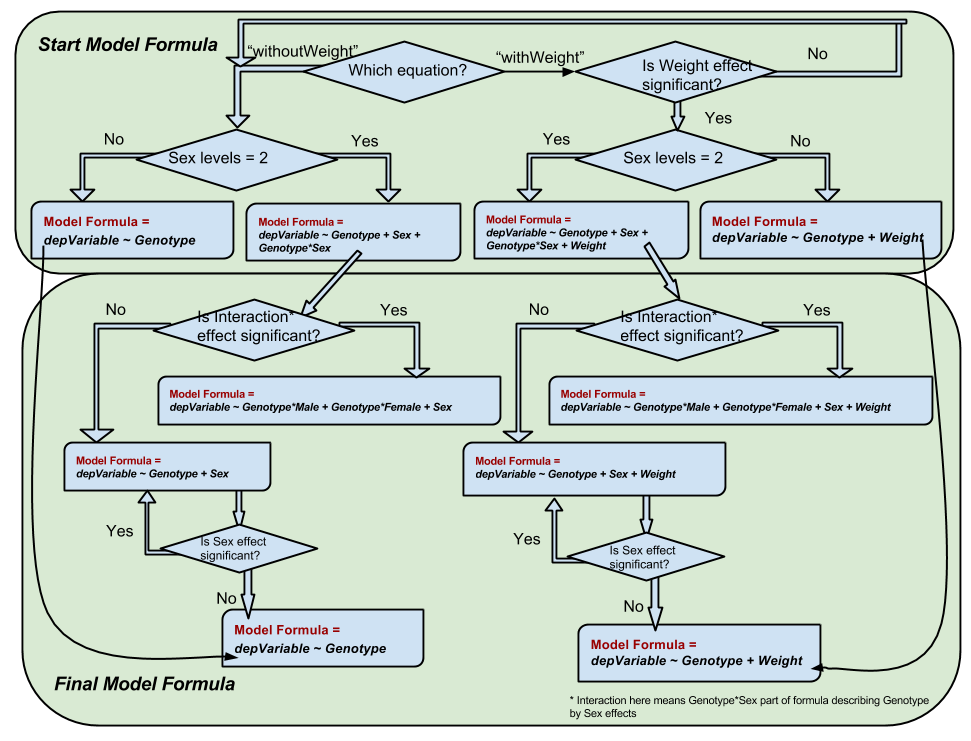
\includegraphics[scale=0.5]{Model_Formula.png}}
\caption{MM framework: start model formula and final model formula creation based on the dataset and significances of the effects (can be estimated or defined by user). }\label{fig:03}
\end{figure}

\begin{figure}[!tpb]%figure04
\centerline{\includegraphics[scale=0.5]{Mixed_Models.png}}
\caption{MM framework: different models that are considered. }\label{fig:04}
\end{figure}

When the final model is selected and reduced, the genotype effect is assessed by comparing a genotype and null model fitted with maximum likelihood evaluation method (ML). Finally, the final genotype model is refitted using restricted maximum likelihood evaluation method (REML) to get unbiased estimates of the variance parameters (see Figure \ref{fig:02} Step 5,6 and Figure \ref{fig:03}).   

\subsubsection{Implementation}
\label{sec:MMImplementation}
There are two functions in the PhenStat package that implements the mixed model framework:
\begin{itemize}
\item \textit{startModel} function evaluates model's criteria and stores the result in the \textit{PhenTestResult} object;
\item \textit{finalModel} function builds the final model using the model's criteria from \textit{PhenTestResult} object and fits the model using restricted maximum likelihood method (REML). 
\end{itemize}

By default, both functions will be called from \textit{testDataset} manager sequentially, that is why \textit{startModel} function's arguments and specific for MM method \textit{testDataset} function's arguments concur.
In the text above we mention \textit{startModel} function's arguments only. 

The equation type is defined by \textit{startModel} function's argument \textit{equation} that can take value "withWeight" which is default one and "withoutWeight". The argument defines the presence or absence of body weight effect in the model (see \ref{Eq1} and \ref{Eq2}). 
In case when there are no body weight records in the dataset \textit{startModel} sets \textit{equation} argument to "withoutWeight" automatically.

\textit{startModel} function creates start fully loaded model and modifies it after testing of different hypothesis. 
As was described in the previous theory section the model view is influenced by the number of criteria. 
Each criteria or effect (body weight effect, residual variances homogeneity, Sex effect, genotype by Sex interaction effect, batch effect) is evaluated individually
and TRUE/FALSE values are assigned to the appropriate sections of \textit{PhenTestResult} object based on evaluation results. 
TRUE value means that effect is significant and will be modelled. FALSE value means deletion of the effect from the model.

The package allows to assign user defined values to the effects of the model. 
If user would like to assign TRUE/FALSE values to the effects of the model that differ from calculated ones then (s)he has to define \textit{keepList} argument of \textit{startModel} functions 
which is a list of TRUE/FALSE values for each one criterion in the following order: is batch effect significant, are residual variances homogeneous, is body weight effect significant, 
is Sex effect significant, is Sex by genotype interaction effect significant. 
For instance, keepList=c(TRUE, TRUE, TRUE, TRUE, TRUE) defines the fully loaded model will all possible fixed effects with homogeneous residual variances; 
in turn keepList=c(FALSE, FALSE, TRUE, TRUE, TRUE) defines the fully loaded model without random effects and with heterogeneous residual variances.

\textit{startModel} function checks user defined effects for consistency (for instance, if there are no "Weight" column in the dataset then weight effect can't be assigned to TRUE, etc.)
and prints out both calculated and user defined effects (only when \textit{outputMessages} argument is set to TRUE) for the user's convenience. Note: user defined effects have a priority over calculated (evaluated) effects.

The result of the \textit{startModel} function is MM start model with reduced non-significant effects stored in the \textit{PhenTestResult} object together with the evaluated or user defined effects.
It is important to mention here the convergency problem. If for some reason, the selected model is failing to converge we simplify it by selecting the similar but simplier model and try to fit again. 
For instance, if model with heterogeneous residuals is not converging then model with homogeneous residuals will be selected.

The next step of MM framework: evaluation of genotype effect and fitting of selected model using REML is implemented in package's function \textit{finalModel}. 
The results are added into the \textit{PhenTestResult} object.  \textit{PhenTestResult} object at the end of the MM framework contains model formula, significances of the effects, genotype evaluation results and model fitting results including effect sizes.

By default both functions (\textit{startModel} and \textit{finalModel}) will be called from \textit{testDataset} manager one after another. 
We've made this logical separation of functionality in order to add more flexibility for the statisticians. 
Basically, it means that a user can check the evaluation of fixed effects and the selected model before final model fitting. 
This kind of "debugging" functionality allows the user to change some of the arguments of functions and start the model building process from scratch if needed.

We believe that the possibility to change mixed models framework behaviour as described above will help users to go deeper into details of the modelling process, 
as well as debug and compare the results from different models. 



\begingroup
    \fontsize{8pt}{12pt}\selectfont
\begin{verbatim}

# Default behaviour
> result <- testDataset(test,depVariable="Bone.Area", equation="withoutWeight")
Information:
Dependent variable: 'Bone.Area'.

Information:
Method: Mixed Model framework.

Information:
Calculated values for model effects are: keepBatch=TRUE, keepVariance=TRUE, 
keepWeight=FALSE, keepSex=TRUE, keepInteraction=FALSE.

Information:
Equation: 'withoutWeight'.

Information:
Perform all MM framework stages: startModel and finalModel

# Perform each step of the MM framework separatly
> result <- testDataset(test,depVariable="Bone.Area", equation="withoutWeight",callAll=FALSE)

Information:
Dependent variable: 'Bone.Area'.

Information:
Method: Mixed Model framework.

Information:
Calculated values for model effects are: keepBatch=TRUE, keepVariance=TRUE, 
keepWeight=FALSE, keepSex=TRUE, keepInteraction=FALSE.

Information:
Equation: 'withoutWeight'.

# Estimated model effects
> result$model.effect.batch
[1] TRUE
> result$model.effect.variance
[1] TRUE
> result$model.effect.weight
[1] FALSE
> result$model.effect.Sex
[1] TRUE
> result$model.effect.interaction
[1] FALSE

> result$numberSexes
[1] 2

# Change the effect values: interaction effect will stay in the model
> result <- testDataset(test,depVariable="Bone.Area", 
equation="withoutWeight",keepList=c(TRUE,TRUE,FALSE,TRUE,TRUE),callAll=FALSE)

Information:
Dependent variable: 'Bone.Area'.

Information:
Method: Mixed Model framework.

Information:
User's values for model effects are: keepBatch=TRUE, keepVariance=TRUE, 
keepWeight=FALSE, keepSex=TRUE, keepInteraction=TRUE.

Information:
Calculated values for model effects are: keepBatch=TRUE, keepVariance=TRUE, 
keepWeight=FALSE, keepSex=TRUE, keepInteraction=FALSE.

Warning:
Calculated values differ from user defined values for model effects.

Information:
Equation: 'withoutWeight'.

> result <- finalModel(result)

> summaryOutput(result)
...
\end{verbatim}
\endgroup

\subsubsection{Diagnostics}
\label{Diagnostics}
There are two functions we've implemented for the diagnostics and classification of MM framework results: \textit{testFinalModel} and \textit{classificationTag}.
 
The first one performs diagnostic tests to assess the MM quality of fit. This includes normality tests for the two genotype levels residuals, BLUPs (best linear unbiased prediction) and 
``rotated'' residuals (\cite{RotatedResiduals04}) (last two only if applicable). There is only one argument of the function which is \textit{PhenTestResult} object. There are no arguments checks assuming that 
function is called internally from the \textit{finalModel} function. Consequently if calling directly it should be used with precaution. 

 \textit{testFinalModel} returns list of the following values:
 \begin{itemize}
  \item Reference genotype value.
  \item Normality test result (p-value) for the reference genotype's residuals.
  \item Test genotype value.
  \item Normality test result (p-value) for the test genotype's residuals.
  \item BLUPs normality test result (p-value); applicable only when there is batch random effects in the model, otherwise set to NA.
  \item ``Rotated'' residuals normality test result (p-value); applicable only when there is batch random effects in the model, otherwise set to NA.
 \end{itemize}

BLUP in statistics is best linear unbiased prediction and is used in linear mixed models for the estimation of random effects. 
See tutorial \href{http://www.extension.org/pages/61006/the-solcap-tomato-phenotypic-data:-estimating-heritability-and-blups-for-traits#.Ui4zjWRgYXc}{BLUPs} for more details.

``Rotated'' residuals are constructed by multiplying the estimated marginal residual vector by
the Cholesky decomposition of the inverse of the estimated marginal variance
matrix. The resulting ``rotated'' residuals are used to construct an empirical cumulative distribution function and pointwise standard errors. See
\href{http://biostats.bepress.com/cgi/viewcontent.cgi?article=1019&context=harvardbiostat}{Cholesky Residuals for Assessing Normal
Errors in a Linear Model with Correlated
Outcomes: Technical Report} for more details about ``rotated'' residuals.

\subsubsection{Classification Tag}
\textit{classificationTag} function returns a classification tag to assign a sexual dimorphism assessment of the phenotypic change from the results of MM framework.
\begingroup
    \fontsize{8pt}{12pt}\selectfont
\begin{verbatim}
> testFinalModel(result)
[1] "+/+"                "0.0560133469740866" "Sparc/Sparc"       
[4] "0.816672883686998"  "0.345325318416593"  "0.0480124939288989"
> classificationTag(result)
[1] "With phenotype threshold value 0.01 - both sexes equally"
\end{verbatim}
\endgroup

When the function is called through \textit{vectorOutput} function,  the tag shown in Figure \ref{fig:05} will be proceeded by the phrase “If phenotype is significant”,  meaning that globally the test has not assessed whether there was a statistical significant difference just that if there was this would be the classification if it was statistically significant.  When the function is called through \textit{summaryOutput} function or directly there is an argument \textit{phenotypeThreshold} (default value is 0.01),  which sets the significance threshold of whether there is a phenotype of interest.  If globally, the analysis indicates there is a statistically significant phenotype then the classification tag is appended to the phrase “With phenotype threshold value XXX”.

\begin{figure}[!tpb]%figure05
\centerline{\includegraphics[scale=0.6]{classificationTagMM2.png}}
\caption{Assigning a classification tag. The output of the mixed model framework is queried to assign a classification tag of how the observed phenotype was observed across the two sexes. Within the decision tree, the question “Is the effect the same for both sexes? “ is asking whether mathematically was there an interaction between the  genotype and Sex. Occasionally the procedure will find that there was a significant interaction but when it comes to identifying how this occurred and quantifying the effect for each Sex,  there is insufficient power.  In this scenario the classification returned states  that it “cannot classify the effect”.}\label{fig:05}
\end{figure}

The Mammalian Phenotype Ontology is under development as a community effort to provide standard terms for annotating mammalian phenotypic data and is housed and managed by the JAXS laboratory (see \href{http://www.informatics.jax.org/searches/MP_form.shtml}{MP ontology}). With the mixed model implementation, the output is very rich and a classification tag can be appended to the MP term to give richer information on the observed phenotype (e.g. abnormal circulating sodium levels – both Sexes equally).  Figure \ref{fig:05_2}, details the decision tree that can be used with the MM output to interpret the results such a ontology term can be discerned and an annotation tag added when appropriate.

\begin{figure}[!tpb]%figure04
\centerline{\includegraphics[scale=0.6]{classificationTagMM_MP.png}}
\caption{Assigning a Mammalian Phenotype (MP) ontology term in the presence of sexual dimorphism. }\label{fig:05_2}
\end{figure}
 
\subsection{Fisher Exact Test Framework}
\label{section:FET}
The Fisher Exact Test is implemented with basic R functions from the stats package after the construction of count matrices (also called chi squared tables) from the dataset. 

Together with count matrices we also calculate percentage matrices and statistics for the chi squared tables (using "vcd" R package "Visualizing Categorical Data").  As a measure of change we calculate the maximum effect sizes. 

From the chi squared table statistical significance is assessed using a Fisher Exact Test whilst the biological significance is estimated by an effect size (see section \ref{FE_EffectSize} for more details).

This is calculated separately for 3 subsets (if there are multiple Sex values in the dataset):
\begin{itemize}
 \item combined dataset (regardless the Sex values),
 \item males only subset,
 \item females only subset.
\end{itemize}

A Fisher Exact Test was chosen as most abnormal phenotype traits are rare event thus the signal is low. Batch is not considered significant because day to day variation does not effect abnormality call for these types of variables.

All results are stored in \textit{PhenTestResult} object:

\begingroup
    \fontsize{8pt}{12pt}\selectfont
\begin{verbatim}
> dataset_cat <- read.csv("./PhenStat/extdata/test_categorical.csv")
> test_cat <- PhenList(dataset_cat,testGenotype="Aff3/Aff3")
 
Warning:
Dataset's column 'Assay.Date' has been renamed to 'Batch' and will be used for the batch effect modeling.

Warning:
Dataset has been cleaned by filtering out records with genotype value 
other than test genotype 'Aff3/Aff3' or reference genotype '+/+'.

Warning:
Dataset's 'Weight' column is missed.
You can define 'dataset.colname.weight' argument to specify column 
for the weight effect modeling. Otherwise you can only use mixed model equation 'withoutWeight'.

Information:
Dataset's 'Genotype' column has following values: '+/+', 'Aff3/Aff3'

Information:
Dataset's 'Sex' column has following value(s): 'Female', 'Male'

> result_cat <- testDataset(test_cat,
 depVariable="Thoracic.Processes",
 method="FE")

Information:
Dependent variable: 'Thoracic.Processes'.

Information:
Method: Fisher Exact Test framework.

> result_cat$depVariable
[1] "Thoracic.Processes"
> result_cat$method
[1] "FE"
> result_cat$numberSexes
[1] 2

# Chi squared table for all data
> result_cat$model.output$count_matrix_all

         +/+ Aff3/Aff3
Abnormal 144        12
Normal   755         1

# Chi squared table for males only records
> result_cat$model.output$count_matrix_male

         +/+ Aff3/Aff3
Abnormal  61         5
Normal   392         1

# Percentage matrix for all data
> result_cat$model.output$percentage_matrix_all

         +/+ Aff3/Aff3 ES change
Abnormal  16        92        76
Normal    84         8        76

# Percentage matrix for females only records
> result_cat$model.output$percentage_matrix_female

         +/+ Aff3/Aff3 ES change
Abnormal  19       100        81
Normal    81         0        81

# Matrix statistics for all data
> result_cat$model.output$stat_all

                    X^2 df   P(> X^2)
Likelihood Ratio 36.466  1 1.5536e-09
Pearson          52.600  1 4.0890e-13

Phi-Coefficient   : 0.24 
Contingency Coeff.: 0.234 
Cramer's V        : 0.24 

# Matrix statistics for males only records
> result_cat$model.output$stat_male

                    X^2 df  P(> X^2)
Likelihood Ratio 14.610  1 1.322e-04
Pearson          23.479  1 1.263e-06

Phi-Coefficient   : 0.226 
Contingency Coeff.: 0.221 
Cramer's V        : 0.226 

# Effect size for all data
> result_cat$model.output$ES

[1] 76

# Effect size for females only records
> result_cat$model.output$ES_female

[1] 81

# Fisher Exact Test results for all data
> result_cat$model.output$all

	Fisher's Exact Test for Count Data

data:  count_matrix_all 
p-value = 4.844e-09
alternative hypothesis: true odds ratio is not equal to 1 
95 percent confidence interval:
 0.0003770171 0.1096287774 
sample estimates:
odds ratio 
 0.0159923
 
# p-value for all data
> result_cat$model.output$all$p.value

[1] 4.844291e-09
\end{verbatim}
\endgroup

The same data as shown in examples can be obtained by using output functions of the package: \textit{summaryOutput}, \textit{vectorOutput} and \textit{vectorOutputMatrices}. See section \ref{section:Results} for more details.

If there is only one level for the dependent variable in the dataset e.g. "Normal`` then the package will add level "Other'' into the count matrices for consistency. All values for this level will be set to 0.
The following is an example of such case:
\begingroup
    \fontsize{8pt}{12pt}\selectfont
\begin{verbatim}
> test2 <- PhenList(dataset=read.csv("test_categorical_normal.csv"),
> result2 <- testDataset(test2,depVariable="Thoracic.Processes", method="FE")
> levels(result2$model.dataset$Thoracic.Processes)
[1] "Normal"
> summaryOutput(result2)

Test for dependent variable: Thoracic.Processes
Method: Fisher Exact Test framework

Model output:
All data p-val: 1
All data effect size: 0%
Males only p-val: 1
Males only effect size: 0%
Females only p-val: 1
Females only effect size: 0%

Matrix 'all':
       +/+ Aff3/Aff3
Normal 895        13
Other    0         0

Percentage matrix 'all' statistics:
       +/+ Aff3/Aff3 ES change
Normal 100       100         0
Other    0         0         0

...
\end{verbatim}
\endgroup
\subsubsection{Classification Tag}
We've implemented the function \textit{classificationTag} also for the FE framework. 
However, in the case of Fisher Exact Test it is not sexual dimorphism classification, but rather the overall estimation of the signals significance.

In the Table \ref{table:06} classification tags and observed p-values classification is based on are presented.  The default value of "phenotypeThreshold" is 0.01. In such a case X=0.01

\begin{table}[!h]
\begin{center}
\begin{tabular}{| l | l | l | p{8cm} |}
  \hline
Males only&Females only&All&Classification Tag for X threshold\\\hline
$\textless$ X&$\textless$ X &$\textless$ X&Significant in males, females and in combined dataset\\
$\textless$ X&$\geq$ X&$\textless$ X&Significant in males and in combined dataset\\
$\textless$ X&$\textless$ X&$\geq$ X&Significant in males and in females datasets\\
$\textless$ X&$\geq$ X&$\geq$ X&Significant in males dataset only\\
$\geq$ X&$\textless$ X&$\textless$ X&Significant in females and in combined dataset\\
$\geq$ X&$\textless$ X&$\geq$ X&Significant in females dataset only\\
$\geq$ X&$\geq$ X&$\textless$ X&Significant in combined dataset only\\
$\geq$ X&$\geq$ X&$\geq$ X&Not significant\\
$\textless$ X&NA&$\textless$ X&Significant for the sex tested\\
NA&$\textless$ X&$\textless$ X&Significant for the sex tested\\

\hline  
\end{tabular}
\caption{p-values from Fisher Exact Tests and classification tag. The default value of "phenotypeThreshold" is 0.01. In such a case X=0.01.}\label{table:06}
\end{center}
\end{table}

\section{Output of Results}
\label{section:Results}
The PhenStat package stores the results of statistical analyses in the \textit{PhenTestResult} object.  
For numeric summary of the analysis, there are two functions to present \textit{PhenTestResult} object data to the user: 
\textit{summaryOutput} that provides a printed summary output and \textit{vectorOutput} that creates a vector form output. 
These output forms were generated for differing users needs. 

\subsection{Summary Output}
\label{SummaryOutput}
The \textit{summaryOutput} function supports interactive analysis of the data and prints results on the screen.

The following is an example of summary output of MM framework:
\begingroup
    \fontsize{8pt}{12pt}\selectfont
\begin{verbatim}
 # Mixed Model framework
> test <- PhenList(dataset=read.csv("./PhenStat/extdata/test.csv"),
            testGenotype="Sparc/Sparc",outputMessages=FALSE)
> result <- testDataset(test,
            depVariable="Lean.Mass",outputMessages=FALSE)
> summaryOutput(result)

Test for dependent variable: Lean.Mass
Method: Mixed Model framework

Was batch significant? TRUE
Was variance equal? FALSE
Was there evidence of sexual dimorphism? no (p-value 0.102)
Final fitted model: Lean.Mass ~ Genotype + Sex + Weight
Model output:
Genotype effect: 0.371508943
Classification tag: With phenotype threshold value 0.01 - no significant change
                         Value  Std.Error  DF    t-value      p-value
(Intercept)          7.6111388 0.58862654 411 12.9303357 2.512303e-32
GenotypeSparc/Sparc -0.2914357 0.33047985 411 -0.8818562 3.783700e-01
SexMale           1.6407343 0.18080930 411  9.0743913 4.791912e-18
Weight               0.3430502 0.01808121 411 18.9727422 4.147891e-58
\end{verbatim}
\endgroup

The summary output for MM framework contains metrics indicating the quality of the fit:
\begin{itemize}
\item \textbf{Intercept} is the reference level after all other factors are accounted for. For example, for equation with weight (\ref{Eq2}) in fully loaded model intercept is reference genotype's female with zero weight. 
 \item \textbf{Value} stands for the estimated coefficient. This number will obviously vary based on the magnitude of the variable your are inputting into the regression, but it's always good to spot check this number to make sure it seems reasonable.

\item \textbf{Std.Error} is a standard error of the coefficient estimate -- measure of the variability in the estimate for the coefficient. Lower is better but this number is relative to the value for the coefficient. 

\item \textbf{DF} stands for the ``Degrees of Freedom'' which is the difference between the number of observations included in training sample and the number of variables used in model (intercept counts as a variable).

\item \textbf{t-value} of the coefficient estimate is a score that measures whether or not the coefficient for this variable is meaningful for the model. It is used to calculate the p-value.

\item \textbf{p-value} is variable p-value that represents the probability the variable is NOT relevant. The smaller is number the more important is variable (model part). If the number is really small, R will display it in scientific notation.
\end{itemize}

For the "FE" framework results \textit{summaryOutput} function's output includes count matrices, statistics and effect size measures.

\begingroup
    \fontsize{8pt}{12pt}\selectfont
\begin{verbatim}
test2 <- PhenList(dataset=read.csv("./PhenStat/extdata/test_categorical.csv"),
            testGenotype="Aff3/Aff3",outputMessages=FALSE)
result2 <- testDataset(test2,
            depVariable="Thoracic.Processes",
            method="FE",outputMessages=FALSE)  
summaryOutput(result2)

Test for dependent variable: Thoracic.Processes
Method: Fisher Exact Test framework

Model output:
All data p-val: 4.84429148175386e-09
All data effect size: 76%
Males only p-val: 0.000286667802768362
Males only effect size: 70%
Females only p-val: 1.00779809539594e-05
Females only effect size: 81%

Matrix 'all':
         +/+ Aff3/Aff3
Abnormal 144        12
Normal   755         1

Percentage matrix 'all' statistics:
         +/+ Aff3/Aff3 ES change
Abnormal  16        92        76
Normal    84         8        76

Matrix 'all' statistics:
                    X^2 df   P(> X^2)
Likelihood Ratio 36.466  1 1.5536e-09
Pearson          52.600  1 4.0890e-13

Phi-Coefficient   : 0.24 
Contingency Coeff.: 0.234 
Cramer's V        : 0.24 

Matrix 'males only':
...
\end{verbatim}
\endgroup

\subsection{Vector Format}
\textit{vectorOutput} function was developed for large scale application where automatic implementation would be required. 
As such, each value within the output vector is strictly defined and depends only on the statistical analysis method that has been used. 
The main idea here is that vector format is specified and is the same regardless the analysis framework.

\begingroup
    \fontsize{8pt}{12pt}\selectfont
\begin{verbatim}Genotype
> vectorOutput(result)
                                          Method 
"MM framework, linear mixed-effects model, equation with weight" 
                                Dependent variable 
                                       "Lean.Mass" 
                                    Batch included 
                                            "TRUE" 
                    Residual variances homogeneity 
                                           "FALSE" 
                             Genotype contribution 
                               "0.371508943144266" 
                                 Genotype estimate 
                               "-0.29143571549456" 
                           Genotype standard error 
                               "0.330479850268177" 
                                    Genotype p-val 
                               "0.378369997588029" 
                                   Sex estimate 
                                "1.64073430331594" 
                             Sex standard error 
                               "0.180809296427475" 
                                      Sex p-val 
                            "4.79191190571249e-18" 
                                   Weight estimate 
                               "0.343050209791982" 
                             Weight standard error 
                              "0.0180812139273457" 
                                      Weight p-val 
                             "4.1478905048872e-58" 
...
\end{verbatim}
\endgroup


In the Table \ref{table:07} vector output values are described.
\begin{sidewaystable}
 
\begin{tabular}{| l | l | l | l | p{10cm} |}
  \hline
\#&Name&Value&Framework&Description\\\hline
1&Method&String&MM and FE&Possible values: "FE", "MM, linear mixed-effects model/generalized least squares, equation with weight/equation without weight".\\
2&Dependent variable&String&MM and FE&Name of the dependent variable.\\
3&Batch included&TRUE/FALSE&MM&Was batch significant in MM?\\
4&Residual variances homogeneity&TRUE/FALSE&MM&Was variance equal in MM?\\
5&Genotype contribution&Numeric&MM and FE&p-value indicating genotype contribution.\\
6&Genotype estimate&Numeric&MM and FE&Estimated coefficient that describes genotype value calculated by MM or effect size estimates in FE.\\
7&Genotype standard error&Numeric&MM&Standard error of the coefficient estimate for genotype in MM.\\
8&Genotype p-val&Numeric&MM&Genotype p-value that represents the probability the genotype is NOT relevant in MM.\\
9&Sex estimate&Numeric&MM&Estimated coefficient that describes Sex value calculated by the MM.\\
10&Sex standard error&Numeric&MM&Standard error of the coefficient estimate for Sex in MM.\\
11&Sex p-val&Numeric&MM&Sex p-value that represents the probability the Sex is NOT relevant in MM.\\
12&Weight estimate&Numeric&MM&Estimated coefficient that describes weight value calculated by the MM.\\
13&Weight standard error&Numeric&MM&Standard error of the coefficient estimate for weight in MM.\\
14&Weight p-val&Numeric&MM&Weight p-value that represents the probability the weight is NOT relevant in MM.\\
15&Gp1 genotype&String&MM and FE&Value of reference genotype.\\
16&Gp1 Residuals normality test&Numeric&MM&p-value that represents the probability the residuals in reference genotype subset are normally distributed.\\
17&Gp2 genotype&String&MM and FE&Value of test genotype.\\
18&Gp2 Residuals normality test&Numeric&MM&p-value that represents the probability the residuals in test genotype subset are normally distrbuted.\\
19&Blups test&Numeric&MM&p-value that represents the probability the blups are normally distrbuted.\\
\hline  
\end{tabular}
\end{sidewaystable}

\begin{sidewaystable}
 
\begin{tabular}{| l | l | l | l | p{10cm} |}
  \hline
\#&Name&Value&Framework&Description\\\hline
20&Rotated residuals normality test&Numeric&MM&p-value that represents the probability the rotated residuals are normally distrbuted.\\
21&Intercept estimate&Numeric&MM&Estimated coefficient that describes intercept value calculated by the MM.\\
22&Intercept standard error&Numeric&MM&Standard error of the coefficient estimate for intercept in MM.\\
23&Interaction included&TRUE/FALSE&MM&Indicates the inclusion of genotype by Sex interaction effect into MM.\\
24&Interaction p-val&Numeric&MM&Interaction p-value that represents the probability the interaction is NOT relevant in MM.\\
25&Sex FvKO estimate&Numeric&MM and FE&Estimated coefficient that describes value calculated by the MM for females in test genotype subset or effect size estimate calculated from chi table for females only subset in FE.\\
26&Sex FvKO standard error&Numeric&MM&Standard error of the "Sex FvKO estimate" in MM.\\
27&Sex FvKO p-val&Numeric&MM&p-value that represents the probability that females group from test genotype subset contribution into MM is NOT relevant.\\
28&Sex MvKO estimate&Numeric&MM and FE&Estimated coefficient that describes value calculated by the MM for males in test genotype subset or effect size estimate calculated from chi table for males only subset in FE.\\
29&Sex MvKO standard error&Numeric&MM&Standard error of the "Sex MvKO estimate" in MM.\\
30&Sex MvKO p-val&Numeric&MM&p-value that represents the probability that males group from test genotype subset contribution into MM is NOT relevant.\\
31&Classification tag&String&MM and FE&A sexual dimorphism assessment of the phenotypic change from the results of MM or the overall estimation of the signals significance in FE.\\
32&Additional information&String&MM and FE&Additional info concerning dataset, for instance, subsets sizes for MM. String in JSON format.\\
\hline  
\end{tabular}
\caption{Vector output description.}\label{table:07}
\end{sidewaystable}

As was mentioned above \textit{vectorOutput} format is the same for both frameworks. However, in case of "FE" many values are not defined. For example:

\begingroup
    \fontsize{8pt}{12pt}\selectfont
\begin{verbatim}
> vectorOutput(result_cat)

                                                 Method 
                                    "Fisher Exact Test" 
                                     Dependent variable 
                                   "Thoracic.Processes" 
                                         Batch included 
                                                     NA 
                         Residual variances homogeneity 
                                                     NA 
                                  Genotype contribution 
                                                     NA 
                                      Genotype estimate 
                                                   "76" 
                                Genotype standard error 
                                                     NA 
                                         Genotype p-val 
                                 "4.84429148175386e-09" 
                                        Sex estimate 
                                                     NA 
                                  Sex standard error 
                                                     NA 
                                           Sex p-val 
                                                     NA 
                                        Weight estimate 
                                                     NA 
                                  Weight standard error 
                                                     NA 
                                           Weight p-val 
                                                     NA 
                                           Gp1 genotype 
                                                  "+/+" 
                           Gp1 Residuals normality test 
                                                     NA 
                                           Gp2 genotype 
                                            "Aff3/Aff3" 
                           Gp2 Residuals normality test 
                                                     NA 
                                             Blups test 
                                                     NA 
                       Rotated residuals normality test 
                                                     NA 
                                     Intercept estimate 
                                                     NA 
                               Intercept standard error 
                                                     NA 
                                   Interaction included 
                                                     NA 
                                      Interaction p-val 
                                                     NA 
                                   Sex FvKO estimate 
                                                   "81" 
                             Sex FvKO standard error 
                                                     NA 
                                      Sex FvKO p-val 
                                 "1.00779809539594e-05" 
                                   Sex MvKO estimate 
                                                   "70" 
                             Sex MvKO standard error 
                                                     NA 
                                      Sex MvKO p-val 
                                 "0.000286667802768362" 
                                     Classification tag 
													NA
								Additional information
													NA
\end{verbatim}
\endgroup

\subsection{Count Matrices in Vector Format}
There is an additional function to support the FE framework: \textit{vectorOutputMatrices}. This function returns values from count matrices in the vector format.
We've limited the number of levels for dependent variable to 10. 
In the vector, the first three positions represent: dependent variable, genotype level 1 (reference genotype) and genotype level 2 (test genotype).
The next 10 positions are used to define the dependent variable levels. When there are less than 10 levels, ``NA'' value is used.
The next 20 positions represent combined count matrix values. Thereafter the vector contains the males only count matrix values and females only count matrix values. Again ``NA'' is used when the values are not present. The positions are labelled with the group and level.

For the chi squared tables from example described in ``Fisher Exact Test framework'' subsection (see \ref{section:FET}) results of \textit{vectorOutputMatrices} function look like this:
\begingroup
    \fontsize{8pt}{12pt}\selectfont
\begin{verbatim}
> vectorOutputMatrices(result_cat)
              Dependent variable                Gp1 Genotype (g1) 
            "Thoracic.Processes"                            "+/+" 
               Gp2 Genotype (g2)   Dependent variable level1 (l1) 
                     "Aff3/Aff3"                       "Abnormal" 
  Dependent variable level2 (l2)   Dependent variable level3 (l3) 
                        "Normal"                               NA 
  Dependent variable level4 (l4)   Dependent variable level5 (l5) 
                              NA                               NA 
  Dependent variable level6 (l6)   Dependent variable level7 (l7) 
                              NA                               NA 
 Dependent variable level18 (l8)        Dependent variable level9 
                              NA                               NA 
Dependent variable level10 (l10)                      Value g1_l1 
                              NA                            "144" 
                     Value g2_l1                      Value g1_l2 
                            "12"                            "755" 
                     Value g2_l2                      Value g1_l3 
                             "1"                               NA 
                     Value g2_l3                      Value g1_l4 
                              NA                               NA 
                     Value g2_l4                      Value g1_l5 
                              NA                               NA 
                     Value g2_l5                      Value g1_l6 
                              NA                               NA 
                     Value g2_l6                      Value g1_l7 
                              NA                               NA 
                     Value g2_l7                      Value g1_l8 
                              NA                               NA 
                     Value g2_l8                      Value g1_l9 
                              NA                               NA 
                     Value g2_l9                     Value g1_l10 
                              NA                               NA 
                    Value g2_l10                 Male Value g1_l1 
                              NA                             "61" 
                Male Value g2_l1                 Male Value g1_l2 
                             "5"                            "392" 
                Male Value g2_l2                 Male Value g1_l3 
                             "1"                               NA 
                Male Value g2_l3                 Male Value g1_l4 
                              NA                               NA 
                Male Value g2_l4                 Male Value g1_l5 
                              NA                               NA 
                Male Value g2_l5                 Male Value g1_l6 
                              NA                               NA 
                Male Value g2_l6                 Male Value g1_l7 
                              NA                               NA 
                Male Value g2_l7                 Male Value g1_l8 
                              NA                               NA 
                Male Value g2_l8                 Male Value g1_l9 
                              NA                               NA 
                Male Value g2_l9                Male Value g1_l10 
                              NA                               NA 
               Male Value g2_l10               Female Value g1_l1 
                              NA                             "83" 
              Female Value g2_l1               Female Value g1_l2 
                             "7"                            "363" 
              Female Value g2_l2               Female Value g1_l3 
                             "0"                               NA 
              Female Value g2_l3               Female Value g1_l4 
                              NA                               NA 
              Female Value g2_l4               Female Value g1_l5 
                              NA                               NA 
              Female Value g2_l5               Female Value g1_l6 
                              NA                               NA 
              Female Value g2_l6               Female Value g1_l7 
                              NA                               NA 
              Female Value g2_l7               Female Value g1_l8 
                              NA                               NA 
              Female Value g2_l8               Female Value g1_l9 
                              NA                               NA 
              Female Value g2_l9              Female Value g1_l10 
                              NA                               NA 
             Female Value g2_l10 
                              NA 
\end{verbatim}
\endgroup                            
\section{Graphics}
For graphical output of the analysis, multiple graphical functions have been generated and these can be called by a user individually or alternatively, 
\textit{generateGraphs} generates all relevant graphs for an analysis and stores the graphs in the defined directory. 

\begingroup
    \fontsize{8pt}{12pt}\selectfont
\begin{verbatim}
> generateGraphs(phenTestResult=result,dir="./graphs",graphingName="Lean Mass",type="windows")

> generateGraphs(phenTestResult=result_cat,dir="./graphs_categorical",type="windows")
\end{verbatim}
\endgroup 

\subsection{Graphics for Categorical Data}
There is only one graphical output for FE framework: categorical bar plots. This graph allows a visual representation of the count data, comparing observed proportions between reference and test genotypes.  

\begingroup
    \fontsize{8pt}{12pt}\selectfont
\begin{verbatim}
> categoricalBarplot(result_cat)
\end{verbatim}
\endgroup 

The example of bar plot is shown in Figure \ref{fig:06}. This graph allows a visual representation of the genotype effect for the variable of interest.
\begin{figure}[!htpb]%figure01
\centerline{\includegraphics[scale=0.5]{categoricalBarPlot.png}}
\caption{The PhenStat package's graphical output: categorical bar plot.}\label{fig:06}
\end{figure}

\subsection{Graphics for Continuous Data}
There are many graphic functions for the MM framework results. They can be divided into two types: dataset based graphs and results based graphs.
There are three functions in the dataset based graphs category:
\begin{itemize}
\item \textit{boxplotSexGenotype} creates a box plot split by Sex and genotype.
\item \textit{boxplotSexGenotypeBatch} creates a box plot split by Sex, genotype and batch if batch data present in the dataset. Please note the batches are not ordered with time but allow assessment of how the treatment groups lie relative to the normal control variation.
\item \textit{scatterplotGenotypeWeight} creates a scatter plot body weight versus dependent variable. Both a regression line and a loess line (locally weighted line) is fitted for each genotype.
\end{itemize}

\begingroup
    \fontsize{8pt}{12pt}\selectfont
\begin{verbatim}
> boxplotSexGenotype(test,depVariable="Lean.Mass",graphingName="Lean Mass")
> boxplotSexGenotypeBatch(test,depVariable="Lean.Mass",graphingName="Lean Mass")
> scatterplotGenotypeWeight(test,depVariable="Bone.Mineral.Content",graphingName="BMC")
\end{verbatim}
\endgroup 

An example of box plot split by Sex and genotype is shown in Figure \ref{fig:07}. Outliers are shown as independent data points beyond the fences (``whiskers'') of the boxplot. An outlier is defined as a data point that is 1.5 times the interquartile range above the upper quartile and bellow the lower quartile.
\begin{figure}[!htpb]%figure01
\centerline{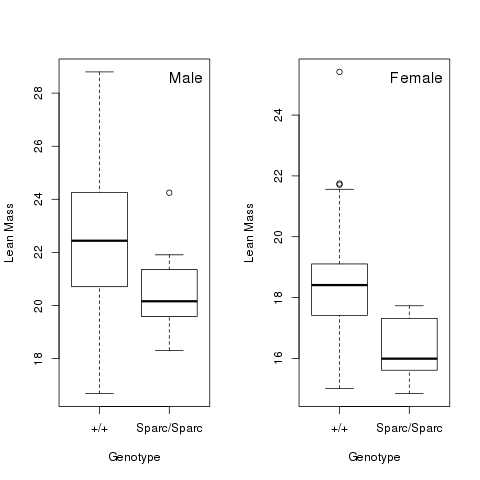
\includegraphics[scale=0.5]{boxplotSexGenotype.png}}
\caption{The PhenStat package's graphical output: box plot split by Sex and genotype.}\label{fig:07}
\end{figure}

The example of box plot split by Sex, genotype and batch is shown in Figure \ref{fig:08}. This allows a visualisation of variation of dependent variable with time. The MM framework assumes this variation is random and conforms the normal distribution. Then the genotype distribution can be compared relative to natural variation. 
\begin{figure}[!htpb]%figure01
\centerline{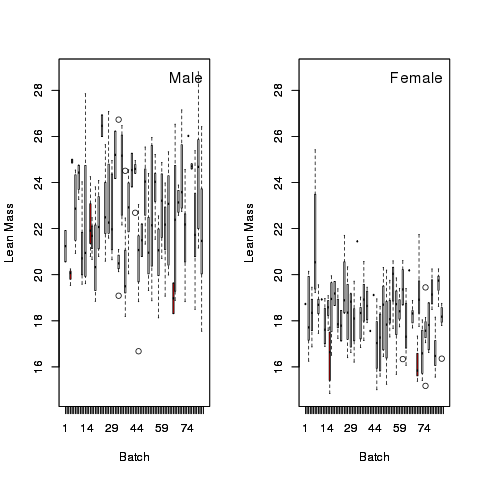
\includegraphics[scale=0.5]{boxplotSexGenotypeBatch.png}}
\caption{The PhenStat package's graphical output: box plot split by Sex, genotype and batch.}\label{fig:08}
\end{figure}

The example of scatter plot of body weight versus dependent variable is shown in Figure \ref{fig:09}. When weight is included in the model MM framework, it assumes a linear relationship between dependent variable and body weight. This graph allows an assessment of this assumption. 
\begin{figure}[!htpb]%figure01
\centerline{\includegraphics[scale=0.5]{scatterplotGenotypeWeight.png}}
\caption{The PhenStat package's graphical output: scatter plot of body weight versus dependent variable.}\label{fig:09}
\end{figure}

There are five functions in the results based graphs category:
\begin{itemize}
\item \textit{qqplotGenotype} creates a Q-Q plot of residuals for each genotype.
\item \textit{qqplotRandomEffects} creates a Q-Q plot of blups (best linear unbiased predictions).
\item \textit{qqplotRotatedResiduals} creates a Q-Q plot of ``rotated'' residuals.
\item \textit{plotResidualPredicted} creates predicted versus residual values plots split by genotype.
\item \textit{boxplotResidualBatch} creates a box plot with residue versus batch split by genotype.
\end{itemize}

\begingroup
    \fontsize{8pt}{12pt}\selectfont
\begin{verbatim}
> qqplotGenotype(result)
> qqplotRandomEffects(result)
> qqplotRotatedResiduals(result)
> plotResidualPredicted(result)
> boxplotResidualBatch(result)
\end{verbatim}
\endgroup 

The example of Q-Q plot of residuals for each genotype is shown in Figure \ref{fig:10}. The MM framework assumes residuals are normally distributed. Residuals are the differences between the real values observed for a dependent variable and the fitted values from the model. A Q-Q plot assesses this assumption (residuals will be randomly arranged around the line if normally distributed). 
\begin{figure}[!tpb]%figure01
\centerline{\includegraphics[scale=0.5]{qqplotGenotype.png}}
\caption{The PhenStat package's graphical output: Q-Q plot of residuals for each genotype.}\label{fig:10}
\end{figure}


The example of Q-Q plot of BLUPs (best linear unbiased predictions) is shown in Figure \ref{fig:11}. The MM framework assumes the BLUPs are normally distributed. This graph assesses this assumption by plotting BLUPs and the ideal normal line (large deviations from the line can be an indicator of problems with the model fit). BLUPs are best linear unbiased predictions and are used for the estimation of batch effects. See tutorial \href{http://www.extension.org/pages/61006/the-solcap-tomato-phenotypic-data:-estimating-heritability-and-blups-for-traits#.Ui4zjWRgYXc}{BLUPs} for more details.

\begin{figure}[!htpb]%figure01
\centerline{\includegraphics[scale=0.5]{qqplotRandomEffects.png}}
\caption{The PhenStat package's graphical output: Q-Q plot of BLUPs (best linear unbiased predictions).}\label{fig:11}
\end{figure}

Another method to assess the model fit is to consider the normality of the ``rotated'' and ``unrotated'' residuals. The example of Q-Q plot of ``rotated'' residuals is shown in Figure \ref{fig:12}. 
See section \ref{Diagnostics} for the details about ``rotated'' residuals.

\begin{figure}[!htpb]%figure01
\centerline{\includegraphics[scale=0.5]{qqplotRotatedResiduals.png}}
\caption{The PhenStat package's graphical output: Q-Q plot of ``rotated'' residuals.}\label{fig:12}
\end{figure}

The example of residual-by-predicted plot is shown in Figure \ref{fig:13}. Residuals, differences between fitted and real values, are plotted against the predicted (fitted) values of dependent variable.  
A residual-by-predicted plot can be used to diagnose nonlinearity or nonconstant error variance. It is also can be used to find outliers. 

Here are the characteristics of a residual-by-predicted plot when model fitness is close to the ideal and what they suggest about the appropriateness of the model:
\begin{itemize}
\item The residuals are arranged randomly around the 0 line. This suggests that the assumption that the relationship is linear is reasonable.
\item The residuals roughly form a "horizontal band" around the 0 line. This suggests that the variances of the error terms are equal.
\item No one residual outstands from the basic random pattern of residuals. This suggests that there are no outliers. See \href{https://onlinecourses.science.psu.edu/stat501/node/36}{Regression Methods} for more details.
\end{itemize}
\begin{figure}[!htpb]%figure01
\centerline{\includegraphics[scale=0.5]{plotResidualPredicted.png}}
\caption{The PhenStat package's graphical output: residual-by-predicted plot split by genotype.}\label{fig:13}
\end{figure}

The example of box plot with residue versus batch split by genotype is shown in Figure \ref{fig:14}. This allows assessment that the residual behaviour for all batches is within natural deviation and the model is fitting the data well.
\begin{figure}[!htpb]%figure01
\centerline{\includegraphics[scale=0.5]{boxplotResidualBatch.png}}
\caption{The PhenStat package's graphical output: box plot with residual versus batch split by genotype.}\label{fig:14}
\end{figure}
   
\section{Case Studies}
\subsection{PhenStat Usage Example Continuous Data}
The following dataset, provided by Wellcome Trust Sanger Institute (WTSI) Mouse Genetics Project (\href{http://www.sanger.ac.uk/resources/mouse/}{MGP}) 
is Dual-energy X-ray absorptiometry data obtained for a study on gene knockout mice carrying the \textit{Akt2$\textless$tm1Wcs$\textgreater$} targeted allele which were created by blastocyst 
injection of targeted ES cells, and bred on the 129S5\/SvEvBrd genetic background.  
Data was collected doing a standardized high throughput phenotyping pipeline following a multi-batch workflow, where regular control animals are collected and knockout animals of the correct age are issued to the pipeline as they arise.  

\begin{table}[!h]
\begin{center}
\begin{tabular}{| l | l | c | c |}
  \hline
Genotype&Sex&Number Animals&Number Batches\\\hline
\multirow{2}{*}{\textit{Akt2}\slash \textit{Akt2}}&Female&12&3\\
			    &Male&14&3\\
			    \hline
\multirow{2}{*}{+\slash +}&Female&574&96\\
			    &Male&572&97\\

\hline  
\end{tabular}
\caption{Number of animals and number of batches in the \textit{Akt2} dataset}\label{table:08}
\end{center}
\end{table}

\subsubsection{Loading the data and initial steps of analysis}
Initial steps focus on loading the data, using the PhenStat tools to generate the PhenList object, and then the result object.  
We can then explore the data and fitted results using the visualisation and output functions.   
\begingroup
    \fontsize{8pt}{12pt}\selectfont
\begin{verbatim}
> DEXAdata=read.csv("WTSI_AKt2_data.csv")
> test <- PhenList(dataset=DEXAdata,testGenotype="Akt2/Akt2",  
  refGenotype="WT",
  dataset.colname.batch="dateOfExperiment", 
  dataset.values.female="female", 
  dataset.values.male="male" )
> result <- testDataset(test,depVariable="Lean.Mass",method="MM",equation="withoutWeight")
\end{verbatim}
\endgroup 



\subsubsection{Exploring and understanding the output}
\label{cs1_output}
The first two lines of the \textit{summaryOutput} confirm the statistical framework used and the dependent variable studied.   
The next section of the output clarifies the final fitted model details. As the MM framework is an optimisation process exploring the data to fit the best model to the data, 
the final fitted model details will vary. We can see that batch variation, the variation in readings between different assay dates, 
were found to be statistical significant and hence a mixed model will have been fitted where batch is treated as a random effect.  
If it was not significant, then the model would have reverted to a simpler linear model.  
The next line of output, “was variance equal?”, indicating whether the model assumes equal variance between genotype groups or unequal.  
In this case, the variance was not found to be equal and therefore the final model estimated the variance for each group separately. 

The next stage of the output, indicates whether there was evidence of sexual dimorphism (i.e. the genotype effect was found to be dependent on sexes).  
In this case, the statistical test of sexual dimorphism was non-significant (p-value = 0.899) hence the final model assessed a genotype effect rather than the genotypes for each sex separately.  
The following line indicate which main effects were included in the final model; 
for this variable and dataset we can see that Sex was significant in explaining variation in the data and hence is included in the final model. 

The final stage of the output gives information on the final model details.  
The “Genotype effect” reports the statistical significance for the genotype effect and is assessed by comparing a treatment model (final fitted model) with a null model where a null model 
has no genotype effects in the model but all other significant main effects.  
In this example the null model would thus be Lean.Mass $\sim$ Sex. Looking at the output the “Genotype effect” is highly statistical significant as a 0 value is reported.  
We can then look at the model fitting details in the final output of the function by examining the table to see how the main effects contributed to the variation in the dependent variables. 

\begingroup
    \fontsize{8pt}{12pt}\selectfont
\begin{verbatim}
> summaryOutput(result)

Test for dependent variable: Lean.Mass
Method: Mixed Model framework

Was batch significant? TRUE
Was variance equal? FALSE
Was there evidence of sexual dimorphism? no (p-value 0.906)
Final fitted model: Lean.Mass ~ Genotype + Sex
Model output:
Genotype effect: 0
Classification tag: With phenotype threshold value 0.01 - both sexes equally
                      Value Std.Error   DF   t-value       p-value
(Intercept)       18.525264 0.1936360 1048 95.670550  0.000000e+00
GenotypeAkt2/Akt2 -3.527111 0.4866433 1048 -7.247836  8.204401e-13
SexMale         4.620361 0.1581236 1048 29.219943 8.940893e-138

\end{verbatim}
\endgroup 

A regression model estimates each component of the model, by isolating how that effect influences the dependent variable (i.e. lean mass) as though all other parts of the model had been fixed and isolated.   
From the table of output, we can see that the intercept (the expected reading for lean mass for female reference genotype (aka female wild type animals) is 18.5.  
Then we can see the effect of the genotype is -3.5 in that knockout animals are predicted to have 3.5 grams less lean mass relative to the control animals.  
Finally we can see that being a male animals leads to an increase of 4.6 grams.  
As there was no evidence for sexual dimorphism, and thus the genotype effect was estimated independently of Sex, then a classification tag “both sexes equally” has been assigned.  
These estimates are in agreement with the visualisation of the data (see section \ref{AssesingModelFit}). 

\subsubsection{Assessment of raw data and distribution characteristics}
To assess model fit, graphical tools are ideal.  They focus on two areas:
\begin{enumerate}
 \item Assessment of raw data and distribution characteristics
 \item Assessment of model fit
\end{enumerate}
\label{AssesingModelFit}

The function, \textit{boxplotSexGenotype}, allows the genotype effect to be visualised for each Sex group. 
For the \textit{Akt2} example, we can suggest that there looks to be a significant genotype effect that is seen in both Sexes. 
\begingroup
    \fontsize{8pt}{12pt}\selectfont
\begin{verbatim}
> boxplotSexGenotype(result, "Lean.Mass", "Lean Mass (g)")
\end{verbatim}
\endgroup 

\begin{figure}[H]%figure01
\centerline{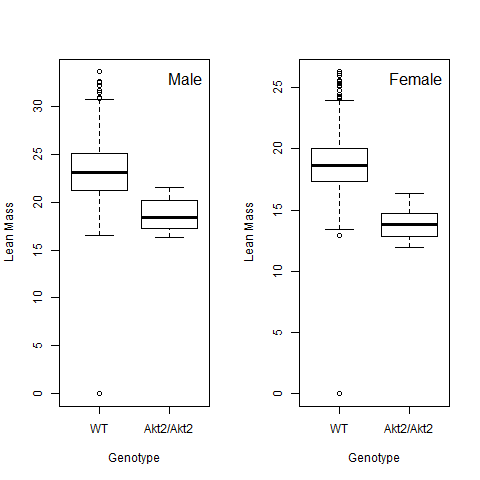
\includegraphics[scale=0.5]{cs1_boxplotSexGenotype.png}}
\caption{\textit{boxplotSexGenotype} function for \textit{Akt2} example.}\label{fig:15}
\end{figure}

A second function, \textit{boxplotSexGenotypeBatch}, allows the comparison between genotype as a function of batch and Sex.  
This plot allows the user to visualise the batch variation and assess how the treatment measures look relative to the batch variation. 
It is important to note that as dates can be entered in many forms, the batches are not ordered with time. 
For the \textit{Akt2} lean mass example, we can see that there is significant batch variation, which explains why a mixed model was fitted.

\begingroup
    \fontsize{8pt}{12pt}\selectfont
\begin{verbatim}
> boxplotSexGenotypeBatch(test, "Lean.Mass", "Lean Mass (g)")
\end{verbatim}
\endgroup 

\begin{figure}[H]%figure01
\centerline{\includegraphics[scale=0.5]{cs1_boxplotBatchGenotype.jpg}}
\caption{\textit{boxplotSexGenotypeBatch} function for \textit{Akt2} example.}\label{fig:16}
\end{figure}

\subsubsection{Assessment of model fit}

Five functions are available and they focus on looking at residual behaviour. 
A residual, is the difference between the estimated dependent variable from the final model estimates and the actual measured dependent variable response. 
A model is a good fit, when the residuals are normally distributed and there is no systematic pattern in the distribution of the residuals relative to the dependent variable. 

The \textit{vectorOutput} function includes statistical tests for normality on the residuals for the wild type, residuals for the knockout, the blups and ``rotated'' residuals (see section \ref{Diagnostics}). 
These normality tests are provide to assist in the building automated tools for assessing model fit, 
however when there is a lot of data (e.g. in a dataset where the wild type arises from a high throughput program with a running baseline), 
the statistical test can be overall sensitive to departures from normality and when the number of data points is low (e.g. in many knockout groups), the test can lack ability to detect deviations from normality. 

\begin{itemize}
 \item \textbf{qqplotGenotype} 
 
This function assesses the normality of the residuals are assessed for each genotype through plotting a normal Q-Q plot. 
Q-Q plots are a means of comparing two distributions. To test normality, we plot the residuals against a normal distribution and see if they match. 
If the two distributions are similar the points on a QQ plot will fall along the y=x line (unity). Thus we are looking for a random distribution of points along the lines.  

Looking at the \textit{Akt2} lean mass example, the residuals on the homozygous knockout group are near perfect showing the model is fitting this data well.  
The residuals on the WT group are deviating in a way (systematic below at one end and systematic above at the other) which indicates that we have long tails to our distribution. 
This is not concerning as we have a very large control dataset and we do have outliers in the data.  

\begingroup
    \fontsize{8pt}{12pt}\selectfont
\begin{verbatim}
> qqplotGenotype(result)
\end{verbatim}
\endgroup 

\begin{figure}[H]%figure01
\centerline{\includegraphics[scale=0.5]{cs1_qqplotGenotype.png}}
\caption{\textit{qqplotGenotype} function for \textit{Akt2} example.}\label{fig:17}
\end{figure}

\item \textbf{boxplotResidualBatch} 

This function allows visualisation to assist the user to assess whether the deviation in the residual is consistent across all the batches and similar in size between the wild type and knockout line. 
For the \textit{Akt2} example, we can see that the variation in residual is consistent across all the batches and similar in size between the knockout and wildtype group.

A few of the wildtype (control) dataset points have large residuals and it would be worth looking at these data points further to see why these are outliers. They do not suggest the model should be discarded because as a proportion of the dataset they are few and scattered through the dataset.

\begingroup
    \fontsize{8pt}{12pt}\selectfont
\begin{verbatim}
> boxplotResidualBatch(result)
\end{verbatim}
\endgroup 

\begin{figure}[H]%figure01
\centerline{\includegraphics[scale=0.5]{cs1_boxplotResidualBatch.png}}
\caption{\textit{boxplotResidualBatch} function for \textit{Akt2} example.}\label{fig:18}
\end{figure}


\item \textbf{plotResidualPredicted} 

This function plots the residuals against the predicted readings for both genotypes.  The predicted readings are the values the model would estimate for the dependent variable.  
As a user, you are looking to see that the model is fitting the data well over the entire data range. 
Looking at the \textit{Akt2} data, we can see that there spread of the residuals is fairly consistent, 
however there are some data points that are not being fit well by the model, the good news is that they are in the control set but they should be considered further to see if a reason for their poor fit can be ascertained.  

\begingroup
    \fontsize{8pt}{12pt}\selectfont
\begin{verbatim}
> plotResidualPredicted(result)
\end{verbatim}
\endgroup 

\begin{figure}[H]%figure01
\centerline{\includegraphics[scale=0.5]{cs1_plotResidualPredicted.png}}
\caption{\textit{plotResidualPredicted} function for \textit{Akt2} example.}\label{fig:19}
\end{figure}

\item \textbf{qqplotRandomEffects} 

This function is assessing the assumption that the batch effects are normally distributed. 
The estimates of the random effects, aka the estimates of the batch effects in this scenario, are called best linear unbiased prediction BLUPs. 
Here a normal Q-Q plot is used to plot the estimated BLUPs against a normal distribution. 
So looking at the \textit{Akt2} lean mass example, the majority of the data points are distrbuted along the line. 
There is some systematic deviation at the tails but it is a small percentage of the points and as it is above and below the line it indicates long tails (ie outliers) 
and so we can conclude the distribution is not too far from the ideal and the model is a good representation of the data. 

\begingroup
    \fontsize{8pt}{12pt}\selectfont
\begin{verbatim}
> qqplotRandomEffects(result)
\end{verbatim}
\endgroup 

\begin{figure}[H]%figure01
\centerline{\includegraphics[scale=0.5]{cs1_qqplotRandomEffects.png}}
\caption{\textit{qqplotRandomEffects} function for \textit{Akt2} example.}\label{fig:20}
\end{figure}

\item \textbf{qqplotRotatedResiduals}

This function, allows the user to consider the normality of the ``rotated'' and ``unrotated'' residuals and have been recommended to assess model fit success with mixed models (\cite{RotatedResiduals04}). 
See section \ref{Diagnostics} for more details. 
So looking at the \textit{Akt2} lean mass example, the majority of the data points are distributed along the line. 
There is some systematic deviation at the tails but it is a small percentage of the points and as it is above and below the line it indicates long tails (i.e. outliers) 
and so we can conclude the distribution is not too far from the ideal and the model is a good representation of the data. 

\begingroup
    \fontsize{8pt}{12pt}\selectfont
\begin{verbatim}
> qqplotRotatedResiduals(result)
\end{verbatim}
\endgroup 

\begin{figure}[H]%figure01
\centerline{\includegraphics[scale=0.5]{cs1_qqplotRotatedResiduals.png}}
\caption{\textit{qqplotRotatedResiduals} function for \textit{Akt2} example.}\label{fig:21}
\end{figure}

\end{itemize}



\subsubsection{Including weight as a covariate in the model fitting process}
Weight is included in the initial model via the \textit{testDataset} function equation argument being set to either “withWeight” or “withoutWeight”.  
When weight is included as a covariate, the model is assuming that the dependent variable (e.g. lean mass) has a linear relationship with body weight. 
If weight is not found to be statistical significant in explaining the variation in the dependent variable, 
then weight as a covariate will drop out of the final model and the equation will automatically revert to an equation type “withoutWeight”.  

There are two advantages to including weight:
\begin{enumerate}
 \item \textbf{Increase in sensitivity.}  
If differences in animal weight lead to greater variability in the dependent variable, then by adding weight and accounting for this variability then the statistical model will be more sensitive to a genotype effect. 

 \item \textbf{Adjusting for weight differences between the knockout and control group.}  
When there is a weight difference between the knockout and wild type animals, the genotype effect is confounded by the weight effect in that there is a difference in the dependent variable but you cannot assess whether it is due to the differences in body weight of the knockout and control animals or genotype differences between the knockout and control animals. When weight is included in the equation, the genotype effect is then testing for a genotype difference after adjusting for the weight difference.

\end{enumerate}

We have found that the majority of continuous phenotypic variables monitored in the WTSI Mouse Genetics Project (\href{http://www.sanger.ac.uk/resources/mouse/}{MGP}) have a relationship with body weight. 
Looking at the \textit{Akt2} dataset we can see that there is a difference in body weight between the wild type and knockout group and thus body weight can be a confounding factor to isolating the genotype effect.   

\begingroup
    \fontsize{8pt}{12pt}\selectfont
\begin{verbatim}
> boxplotSexGenotype(test, "Weight", "Body Weight (g)")
\end{verbatim}
\endgroup 

\begin{figure}[H]%figure01
\centerline{\includegraphics[scale=0.5]{cs1_bodyweight.png}}
\caption{\textit{boxplotSexGenotype} function for \textit{Akt2} example to show the body weight impact.}\label{fig:22}
\end{figure}

When body weight is included, the inclusion can be seen in the final fitted model as weight is listed as a covariate and then in the final model output table, where the influence of weight on the fitted model is shown.  
With weight included the genotype effect is estimating the impact of genotype after adjusting for weight differences in the animals. 

Looking at the \textit{summaryOutput} for the \textit{Akt2} example, the table shows that for each gram of body weight the lean mass increased by 0.32g.  
When weight is included in the equation it changes the definition of the intercept from the lean mass value of a wild type female animal to the lean mass value of a wild type female animal of zero body weight. 
This happens as the model is estimating each of these terms influences in isolation of the other terms. 
In contrast to the earlier fitted results (section \ref{cs1_output}), when weight is included in the model, the classification tag identifies the change as “no significant change” 
as the global genotype test is now not significant with a p-value of 0.64.  
This means the statistically difference observed with the fitted model “withoutWeight” was entirely due to a body weight differences between the knockout and control animals.  
So whilst there is a fundamental differences in lean mass between the knockout and control this is due to the knockout animals being smaller than the control animals. 

\begingroup
    \fontsize{8pt}{12pt}\selectfont
\begin{verbatim}
> summaryOutput(result)

Test for dependent variable: Lean.Mass
Method: Mixed Model framework

Was batch significant? TRUE
Was variance equal? FALSE
Was there evidence of sexual dimorphism? no (p-value 0.105)
Final fitted model: Lean.Mass ~ Genotype + Sex + Weight
Model output:
Genotype effect: 0.639989841
Classification tag: With phenotype threshold value 0.01 - no significant change
                       Value  Std.Error   DF    t-value      p-value
(Intercept)        7.6201046 0.52150631 1047 14.6117207 3.827390e-44
GenotypeAkt2/Akt2 -0.1924952 0.41201772 1047 -0.4672012 6.404531e-01
SexMale         2.1550868 0.17386173 1047 12.3954067 5.056608e-33
Weight             0.3541522 0.01623164 1047 21.8186332 2.718321e-87

\end{verbatim}
\endgroup


\subsubsection{Additional model diagnostics when weight is included}
In addition to the diagnostic discussed in previous section, when weight is included in the model, it is important to consider whether the linear relationship between body weight and the dependent variable is a valid assumption. 
This can be assessed with the \textit{scatterplotGenotypeWeight} function. 
In this plot, for each genotype a regression line is fitted to assess the relationship between the dependent variable and body weight. 
Then a locally weight line (loess line) is plotted. 
The loess line allows assessment that the regression line fits all the data well.
Note the loess line can be distorted by a few data points so if it deviates strongly but for only a few data points, this is not concerning.  
This graph is used to assess whether a linear relationship exists and whether it is the same for both genotypes.  

In the \textit{Akt2} example, it can be clearly seen that a common linear relationship exists between lean mass and body weight, such that as the weight increases so does the lean mass. 
It can also be seen that the knockout animals have a lower body weight and subsequently lower lean mass but the drop in lean mass is entirely in accordance with the drop in body weight. 

\begingroup
    \fontsize{8pt}{12pt}\selectfont
\begin{verbatim}
> scatterplotGenotypeWeight(test, depVariable="Lean.Mass")
\end{verbatim}
\endgroup 

\begin{figure}[H]%figure01
\centerline{\includegraphics[scale=0.5]{cs1_scatterplotGenotypeWeight.png}}
\caption{\textit{scatterplotGenotypeWeight} function for \textit{Akt2} example.}\label{fig:23}
\end{figure}

\subsection{PhenStat Usage Example Categorical Data}
The following dataset, provided by Wellcome Trust Sanger Institute (WTSI) Mouse Genetics Project (\href{http://www.sanger.ac.uk/resources/mouse/}{MGP}) of high resolution X-ray data obtained from 
a study on gene knockout mice carrying the \textit{Aff3tm1a(EUCOMM)Wtsi} targeted allele which were created by blastocyst injection of targeted ES cells, and bred on the B6N genetic background. 
Data was collected on a standardized high throughput phenotyping pipeline following a multi-batch workflow, where regular control animals are collected and knockout animals of the correct age are then issued to the pipeline as they arise. 
At WTSI, batch to batch variation has not been found to be significant for these rare event categorical variables. 
Consequently, we ignore batch and combine data for the same genetic background when collected with the same protocol and housing and husbandry conditions. 
This increases the sensitivity of the analysis as we have more accuracy on the estimate of the prevalence of the condition in the wild type population.

\begin{table}[!h]
\begin{center}
\begin{tabular}{| l | l | c | c |}
  \hline
Genotype&Sex&Number Animals&Number Batches\\\hline
\multirow{2}{*}{\textit{Aff3}\slash \textit{Aff3}}&Female&7&4\\
			    &Male&6&4\\
			    \hline
\multirow{2}{*}{Wild type}&Female&446&70\\
			    &Male&451&70\\

\hline  
\end{tabular}
\caption{Number of animals and number of batches in the \textit{Aff3} dataset}\label{table:09}
\end{center}
\end{table}

\subsubsection{Loading the data and initial steps of analysis}
Initial steps focus on loading the data, using the PhenStat tools to generate the PhenList object, and then the result object.  We can then explore the data and fitted results using the visualisation and output functions.   

\begingroup
    \fontsize{8pt}{12pt}\selectfont
\begin{verbatim}
> aff3data=read.csv("categorical_example 1_aff3_Xray.csv")
> test <- PhenList(dataset=aff3data,testGenotype="Aff3/Aff3", 
  refGenotype="+/+", dataset.colname.batch="Assay.Date")
> result <- testDataset(test, depVariable="Thoracic.Processes", method="FE")
\end{verbatim}
\endgroup 

\subsubsection{Visualisation of data}
The function \textit{categoricalBarplot} has been provided to visualise the categorical data as summary percentage data. 
It reports the percentage of each classification observed for up to three datasets: all data, male only and female only.  
It is important to note that percentage accuracy is very dependent on the number of readings so it is important to consider the dataset size when interpreting these graphs.  
Therefore tables showing both the percentage and count values are included in the \textit{summaryOutput}. 

\begingroup
    \fontsize{8pt}{12pt}\selectfont
\begin{verbatim}
>  categoricalBarplot(result)
\end{verbatim}
\endgroup 

\begin{figure}[H]%figure01
\centerline{\includegraphics[scale=0.5]{cs2_categoricalBarplot.jpg}}
\caption{\textit{categoricalBarplot} function for \textit{Aff3} example.}\label{fig:24}
\end{figure}

\subsubsection{Understanding the \textit{summaryOutput}}

The first two lines of the \textit{summaryOutput} confirm the statistical framework used and the dependent variable studied.  
The next section of the output reports the summary of statistical assessment. Two measures are provided for each dataset considered. 
First a test of statistical significance assessed using a Fisher Exact Test and then a measure of biological significance, the maximum effect size. 
The final section of the output provides tables showing the counts and percentage calculated for each group and possible level. 

The following is reported for dependent variable thoracic processes for the \textit{Aff3} dataset and we can see that for all datasets, there is a statistically significant change with a large effect size. 

The \textit{summaryOutput} function shows the model fitted and the model output for the analysis of the thoracic processes for the \textit{Aff3} dataset. 
The example is showing the summary tables provided for the composite (male and female data) for the thoracic processes for the \textit{Aff3} dataset. 

\begingroup
    \fontsize{8pt}{12pt}\selectfont
\begin{verbatim}
>  summaryOutput(result)

...
Model output:
All data p-val: 4.35745946092922e-09
All data effect size: 76%
Males only p-val: 0.00025633944344021
Males only effect size: 70%
Females only p-val: 1.00779809539594e-05
Females only effect size: 81%

Matrix 'all':
         +/+ Aff3/Aff3
Abnormal 142        12
Normal   753         1

Percentage matrix 'all' statistics:
         +/+ Aff3/Aff3 ES change
Abnormal  16        92        76
Normal    84         8        76

Matrix 'all' statistics:
                    X^2 df   P(> X^2)
Likelihood Ratio 36.678  1 1.3931e-09
Pearson          53.164  1 3.0675e-13

Phi-Coefficient   : 0.242 
Contingency Coeff.: 0.235 
Cramer's V        : 0.242 
...

\end{verbatim}
\endgroup 


\subsubsection{Understanding the maximum effect size reported}
\label{FE_EffectSize}
The maximum effect size is the maximum percentage change seen for an observation type. 
Below is a table showing an artificial example where the majority of the wild type are normal but the abnormality is spread across multiple levels in the knockout. 
For each trait level (i.e. the observed phenotype), the change in percentage effect size is seen by subtracting the percentage observed in the knockout from the wild type. 
Then across all the observed levels, the maximum percentage change is selected after ignoring the direction of the change. 
Thus in the example below, the maximum effect size would be 86.5\% which indicates that there has been 86.5\% change in how often a level is observed.

\begin{table}[!h]
\begin{center}
\begin{tabular}{| l | l | l | l | l | l | l| }
  \hline
\multirow{2}{*}{Trait level}&\multicolumn{2}{c}{wildtype}&\multicolumn{2}{c}{knockout}&\multirow{2}{*}{Effect size calculation}&\multirow{2}{*}{Effect size}\\
		     &count& \%			    &count& \%                   &                                        &\\\hline 
Normal &198& 99			    &1& 12.5                   &          99-12.5                              &86.5\\ 
Abnormal left eye&0& 0			    &0& 0                   &          0                              &0\\ 
Abnormal right eye&1& 0.5			    &4& 50                   &          0.5-50                             &49.5\\ 
Abnormal both eye&1& 0.5			    &3& 37.5                   &          0.5-37.5                             &37\\ 
\hline  
\end{tabular}
\caption{Number of animals and number of batches in the \textit{Aff3} dataset}\label{table:10}
\end{center}
\end{table}

\subsubsection{A dependent variable with little variation}

Within the IMPC pipeline, there are a number of dependent variables which have little variation but are numeric. 
For example, no of digits, or number of caudal vertebrae etc.  
If you try to process these variables through a mixed model framework the analysis will stop and an error will report that there is insufficient variability in the data. 

For our example dataset, the number of ribs is a dependent variable with little variation as shown by plotting the data with the \textit{categoricalBarplot} function.

\begin{figure}[H]%figure01
\centerline{\includegraphics[scale=0.5]{cs2_noRibsRight_percentageplot.jpg}}
\caption{\textit{categoricalBarplot} function for \textit{Aff3} example with number of ribs as dependent variable.}\label{fig:25}
\end{figure}


If we try and process this variable through a mixed model framework the following output is obtained: 


\begingroup
    \fontsize{8pt}{12pt}\selectfont
\begin{verbatim}
> result<-testDataset(test,depVariable="Number.Of.Ribs.Left",method="MM")

Error:
Insufficient variability in the dependent variable 'Number.Of.Ribs.Left' for MM framework. 
Fisher Exact Test can be better way to do the analysis.
Error:
Insufficient variability in the dependent variable 'Number.Of.Ribs.Left' for genotype/Sex 
combinations to allow the application of Mixed Model.
\end{verbatim}
\endgroup 

Instead the dependent variable should be treated as a categorical variable which each numeric output possible treated as a level allowing 
a statistical comparison of how the levels are distributed between the knockout and wildtype groups.  
Thus for our example the following summary output and count table is obtained: 

\begingroup
    \fontsize{8pt}{12pt}\selectfont
\begin{verbatim}
> summaryOutput(result)

Test for dependent variable: Number.Of.Ribs.Left
Method: Fisher Exact Test framework

Model output:
All data p-val: 1
All data effect size: 0%
Males only p-val: 1
Males only effect size: 0%
Females only p-val: 1
Females only effect size: 0%

Matrix 'all':
   +/+ Aff3/Aff3
12   1         0
13 893        13
14   1         0

Percentage matrix 'all' statistics:
   +/+ Aff3/Aff3 ES change
12   0         0         0
13 100       100         0
14   0         0         0

\end{verbatim}
\endgroup 

%\subsection{PhenStat Integration with Database}

\subsection{PhenStat Example Using Cluster}
If someone would like to analyse all variables in the dataset and has a cluster available for such kind of job then here is an example of PhenStat package usage.

First, the function that runs on each cluster's node and stores the results in particular directory is created. This function is based on the section \textit{dataset.stat} of the \textit{PhenList} object. 
\begingroup
\fontsize{8pt}{12pt}\selectfont
\begin{verbatim}
PhenStatCluster<-function(phenList,i){
    # reads variable names from dataset.stat table
    variable <- as.character(phenList$dataset.stat$Variables[i]) 
    
    # checks if variable is continuous again by using dataset.stat table
    isContinuous <- phenList$dataset.stat$Continuous[i]	
    
    # skip the analysis for Batch and Genotype variables
    if (!(variable %in% c("Batch","Genotype"))){	
      if (isContinuous && !(variable %in% c("Weight"))) 
	  # performs MM framework for continuous data
	  result <- testDataset(phenList, variable, method="MM",outputMessages=FALSE)	 
      else
	  if (!isContinuous){
	      # performs FET framework for categorical data
	      result <- testDataset(phenList, variable, method="FE",outputMessages=FALSE)	
	   }
	  else
	      # performs MM framework for weight variable
	      result <- testDataset(phenList, variable, method="MM",equation="withoutWeight",outputMessages=FALSE) 
	      
      write(vectorOutput(result),paste("./",variable,".txt",sep="")) # stores the results
    }
}
\end{verbatim}
\endgroup

We are planning to analyse every individual variable of the dataset using a cluster. Each one cluster node has to have sourced function \textit{PhenStatCluster} and loaded \textit{PhenStat} library. 
\textit{PhenList} object with dataset to analyse should also be available for every cluster node.
\begingroup
\fontsize{8pt}{12pt}\selectfont
\begin{verbatim}
# cluster preparation
# set the folder
setwd("/yourWorkingDirectory")

# create logs folder in it
dir.create(paste(getwd(), "/logs", sep=""))

# define tasks
tasks <- c(1:length(test$dataset.stat$Variables))

# load snow
# snow creates and manages clusters

library(snow)
# create cluster
cluster = makeCluster(length(tasks), type="...") # type values: MPI, RCLOUD, etc.

# Setup cluster nodes
# set current folder on each node
clusterEvalQ(cluster, setwd("/yourWorkingDirectory"))

# create logs and forward output to the log files
clusterEvalQ(cluster, try({ fn = paste(getwd(), "./", Sys.info()[4], "-", Sys.getpid(), ".log", sep=""); 
o <- file(fn, open = "w"); sink(o); sink(o, type = "message"); }))

# test output is routed to the logs
clusterEvalQ(cluster, message("message - OK"))
clusterEvalQ(cluster, cat("cat - OK"))

# load package and source function for each node
clusterEvalQ(cluster, library(PhenStat))
clusterEvalQ(cluster, source("/pathToTheSource/PhenStatCluster.R"))

# export PhenList object to make it available for every node
clusterExport(cluster, "test") 

# finally apply function for each one variable within the dataset
clusterApplyLB(cluster, tasks, function(x){ message("---------- processing ", 
test$dataset.stat$Variables[x], " ----------"); try(PhenStatCluster(test,x)); })

# clean up
stopCluster(cluster)
rm(cluster)
clusterCleanup()
\end{verbatim}
\endgroup

The output is avaialble in the specified directory: 
"/yourWorkingDirectory". 
For each variable from the dataset the output file with results in vector format is created.

\begin{thebibliography}{}

\bibitem[Gentleman \textit{et~al}., 2005]{Gentleman05}
Gentleman,R., Carey,V., Huber,W., Irizarry,R., Dudoit,S.  (2008) Bioinformatics and Computational Biology Solutions Using R and Bioconductor. Springer.  ISBN 978-0-387-25146-2.

\bibitem[Gentleman, 2008]{Gentleman08}
Gentleman,R. (2008) R Programming for Bioinformatics. Chapman \& Hall$\backslash$CRC. ISBN 978-1-4200-6367-7.

\bibitem[Hahne \textit{et~al}., 2008]{Hahne08}
Hahne,F., Huber,W., Gentleman,R., Falcon,S. (2008). Bioconductor Case Studies. Springer.  ISBN 978-0-387-77239-4.

\bibitem[Karp {\it et~al}., 2012]{MM12} Karp,N., Melvin,D., Sanger Mouse Genetics Project, Mott,R. (2012) Robust and Sensitive Analysis of Mouse Knockout Phenotypes, {\it PLoS ONE}, {\bf 7}(12), e52410, doi:10.1371/journal.pone.0052410.

\bibitem[West {\it et~al}., 2007]{MM07}  West,B., Welch,K., Galecki,A. (2007) Linear Mixed Models: A practical guide using statistical software. Chapman \& Hall$\backslash$CRC. ISBN 978-1-584-88480-4.

\bibitem[Houseman {\it et~al}., 2004]{RotatedResiduals04} E. Andrés Houseman, Louise M. Ryan and Brent A. Coull (2004) Cholesky Residuals for Assessing Normal Errors in a Linear Model with Correlated Outcomes, {\it Journal of the American Statistical Association}, {\bf 99} (466), 383-394

\bibitem[Pinkert, 2002]{Pinkert} C.A. Pinkert, Transgenic Animal Technology. A laboratory Handbook (2002), {\it Academic Press Inc.}, USA

%%An R2 statistic for fixed effects in the linear mixed model

%Lloyd J. Edwards1,*, Keith E. Muller2, Russell D. Wolfinger3, Bahjat F. Qaqish1, Oliver Schabenberger3 (2008) DOI: 10.1002/sim.3429
%Statistics in Medicine
%Volume 27, Issue 29, pages 6137–6157, 20 December 2008
\end{thebibliography}


\end{document}